\section{\color{blue}{Effect of Cycles on $\mathcal{H}_2$ performance of Double Integrators}}
%%%%%%%%%%%%%%%%%%%%%%%%%%%%%%%%%%%%%%%%%%%%%%%%%%%%%
\begin{comment}
\begin{frame}{Motivation: The Double Integrator Consensus}
	\vspace{-0.2cm}
	\begin{block}{}
			\textcolor{blue}{The system:}\vspace{-0.3cm} $$\dot{x}_i(t)=v_i(t),~~\dot{v}_i(t)=u_i(t)$$
		\textcolor{blue}{The proposed control law \footnotemark[1]} :
		$u_i(t)=-\sum_{j=1}^{N}{w_{ij}[(x_j(t)-x_i(t))}+\gamma{(v_j(t)-v_i(t))}],$
		
		where $x_i(t),v_i(t)\in \Rp$ denotes position and velocity of the $i^{th}$ agent in a $p$ dimensional space. $w_{ij}$ is the $(i,j)^{\rm th}$ entry of weighted adjacency matrix, and $\gamma$ is called the \textbf{velocity coupling factor}
	\end{block}
\vspace*{-0.2cm}
\begin{block}{}
		Double integrator consensus is achieved if :
	\begin{itemize}
		\item Network has a \emph{spanning tree }for undirected and directed network. [Necessary but not Sufficient]
		\item  $\gamma >0$ for undirected and $\gamma > \max_{i=2,\dots,n}\frac{\Im(\mu_i)}{|\mu_i|\sqrt{{\Re(\mu_i)}}}$for directed network. [Necessary \& Sufficient]~\footnotemark[2]
	\end{itemize}
	where, $\mu_i$, are the non-zero eigenvalues of $\mathcal{L}_n$, where $\Re(.)$ and $\Im(.)$ are the real and imaginary parts respectively.
\end{block}
	%\textcolor{blue}{Consensus} among double integrator, for any initial condition, is defined as:
	\vspace{-0.2cm}
	%\begin{equation*}\label{SecondConsensus}
	%	\begin{array}{ll}
	%		\lim_{t \rightarrow \infty}||x_i(t)-x_j(t)||=0,~~
	%		\lim_{t \rightarrow \infty}||v_i(t)-v_j(t)||=0, ~~ i,j \in \{1,2,\dots,N\}\\
	%	\end{array}
	%\end{equation*}
	%where 
	%\vspace{-0.6cm}
				%\vspace{-0.3cm}
			%\end{equation*}

	%\vspace{0.1cm}
	{\footnotetext[1]{\textcolor{blue}{Ren W, Atkins E}, {\em Second-order consensus protocols in multiple vehicle systems with local interactions}, AIAA guidance, navigation, and control conference and exhibit 2005.}}
	{\footnotetext[2]{\textcolor{blue}{Yu, Wenwu and Chen, Guanrong and Cao, Ming}, {\em Some necessary and sufficient conditions for second-order consensus in multi-agent dynamical systems}, Automatica 2010.}}	
\end{frame}

\end{comment}	
\begin{frame}[noframenumbering]
	\tableofcontents[currentsection]
	%\begin{center}
	%\textcolor{blue}{Problem 2: Effect of cycles on $\mathcal{H}_2$ performance of Double Integrators}
	%\end{center}
\end{frame}


%%%%%%%%%%%%%%%%%%%%%%%%%%%%%%%%%%%%%%%%%%%%%%%%%%%%
\begin{frame}{}
	\vspace{-0.1cm}
		The proposed control law under exogenous input such as node noise and edge noise can be represented as:\vspace{-0.2cm}
%	\vspace*{-0.3cm}
	\begin{equation*}
		u_i(t)=-\sum_{j=1}^{N}{w_{ij}[(x_j(t)-x_i(t))}+\gamma{(v_j(t)-v_i(t))}+r_{ij}(t)]+q_i(t),
	%	\vspace{-0.3cm}
	\end{equation*}
	where, $r_{ij}(t)$ is the edge/measurement noise and $q_i(t)$ is the node noise for $i^{th}$ agent. 
	\vspace{-0.1cm}
		\begin{block}{Noise Characterization}
		-- The node noise is an uncorrelated zero mean Gaussian noise such that $\mathbb{E}[q(t)q^T(t)]=\sigma_{q}^2I_n,$\\
		-- The edge noise is also an uncorrelated zero mean Gaussian noise $\mathbb{E}[r(t)r^T(t)]=\sigma_{r}^2I_e$\\
		where $q(t) \in \R^n$ and $r(t) \in \R^e$, $n,e$ are the number of nodes and edges in a graph and $I_n,I_e$ are identity matrices of dimension $n,e$.
	\end{block}
	\vspace*{-0.2cm}
	\pause
	\begin{block}{Problem Statement}
		Consider a \textcolor{blue}{chain/path of double integrators} following the above consensus protocol. Then,
		\begin{itemize}
			\item Characterize how an exogenous Gaussian noise propagates throughout a system and affect the energy of the monitored output.
			\item How these noises result in asymptotic deviation of each node's state from consensus state. 
			%\item Study effect of cycles on the $\mathcal{H}_2$ performance of the system in context to the combinatorial properties of graph such as cycles.
			%\item Characterize connection between combinatorial properties of graph and the dynamic properties of consensus protocol.
			\item And how does the cycles and $\gamma$ affect the performance of the system measured via the metric $\mathcal{H}_2$ norm.
		\end{itemize}
		%How does the various combinatorial properties of graph such as spanning trees and cycles impact the $\mathcal{H}_2$ performance of the system, in presence of exogenous inputs such as node (process) and edge(measurement) noises.}
		\end{block}
\end{frame}
%%%%%%%%%%%%%%%%%%%%%%%%%%%%%%%%%%%%%%%%%%%%%%%%%%%%
\begin{frame}		
\begin{block}{Literature}
	\begin{itemize}
		%\item Most of the work in the literature are on single integrator and undirected graph.
		\item Zelazo\footnotemark[1], through edge-based analysis, has explored the robustness concerning the combinatorial properties of graphs, albeit still within the context of single integrators and undirected topologies.
		\item The $\mathcal{H}_2$ analysis of networks under directed topology, has been studied by Young\footnotemark[2] for single integrators and by HG Oral\footnotemark[3] for double integrator, but with respect to spectral properties of graph.
		\item $\mathcal{H}_2$ analysis for undirected or directed topology for double integrators has not been explored in context to combinatorial properties of graph.
	\end{itemize}
\end{block}	
\begin{alertblock}{Challenges}
\begin{itemize}
%\item The asymmetrical structure of graph Laplacian in directed networks makes the analysis challenging. 
\item Existence of zero eigenvalues in the Laplacian makes the $\mathcal{H}_2$ norm unbounded.
\item Second Order topology adds further to the complexity.
\end{itemize}
\end{alertblock}
\vspace{0.1cm}
\footnotetext[1]{\textcolor{blue}{Zelazo, Daniel, Simone Schuler, and Frank Allgöwer.}, {\em "Performance and design of cycles in consensus networks." Systems \& Control Letters 62.1 (2013): 85-96.}}
\footnotetext[2]{\textcolor{blue}{Young, George Forrest, Luca Scardovi, and Naomi Ehrich Leonard.}, {\em "Robustness of noisy consensus dynamics with directed communication." Proceedings of the 2010 American Control Conference. IEEE, 2010.}}	
\footnotetext[3]{\textcolor{blue}{Giray Oral, H., Enrique Mallada, and Dennice F. Gayme.}, {\em "Performance of Single and Double-Integrator Networks over Directed Graphs." arXiv e-prints (2019): arXiv-1911.}} 
\end{frame}
%%%%%%%%%%%%%%%%%%%%%%%%%%%%%%%%%%%%%%%%%%%%%%%%%%%%
\begin{frame}{Node dynamics of system in Compact Form}
			\begin{figure}
				\centering
				%\includegraphics[scale=0.3]{blocknoise.png}
				%\includegraphics[trim={1cm 35cm 0cm 7cm},clip,scale=0.16]{block.jpg}
				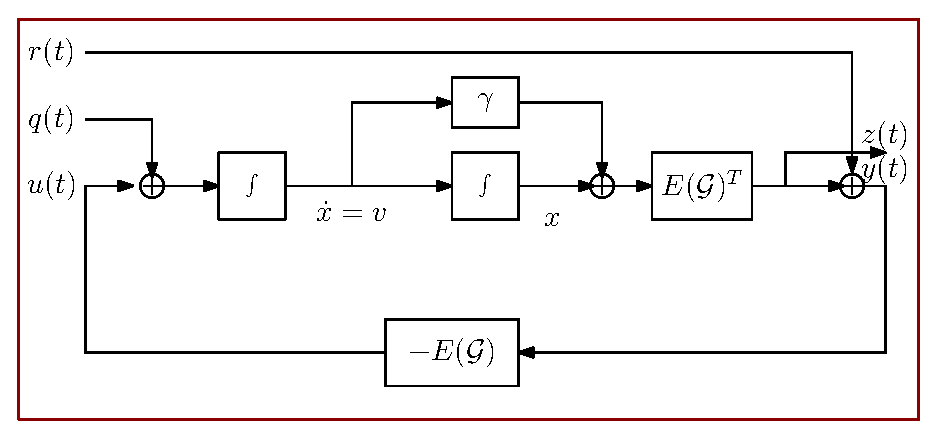
\includegraphics[scale=0.4]{Images/double_int_block_undirected.eps}
			\end{figure}
			\vspace*{-0.25cm}
			\begin{block}{Node Dynamics}
				The node dynamics where $z(t)$ is our monitored performance signal can be written as:
				$$\begin{bmatrix}
					\dot{x} \\ \dot{v}
				\end{bmatrix}=\begin{bmatrix}
					\mathbf{0} & I_n\\
					-\mathcal{L}_n & -\gamma \mathcal{L}_n
				\end{bmatrix}\begin{bmatrix}
					x \\ v
				\end{bmatrix}+
				\begin{bmatrix}
					\mathbf{0} & \mathbf{0}\\
					I_{n} & -E 
				\end{bmatrix}\begin{bmatrix}
					q \\ \r
				\end{bmatrix},~~z(t)=E^Tx(t)+\gamma E^T v(t)$$
				where, $\mathcal{L}_n=EE^T$ is the node Laplacian.
			\end{block}	
			where $x(t)=\begin{bsmallmatrix}x_1,x_2,\dots,x_n \end{bsmallmatrix}^T,v(t)=\begin{bsmallmatrix}v_1,v_2,\dots,v_n \end{bsmallmatrix}^T$ are the agent/node position and velocity vectors,\\
			$q(t)=\begin{bsmallmatrix}q_1,q_2,\dots,q_n \end{bsmallmatrix}^T$ is the node noise and $r(t)=\begin{bsmallmatrix}r_1,r_2,\dots,r_e \end{bsmallmatrix}^T$ is the edge noise
\end{frame}
%%%%%%%%%%%%%%%%%%%%%%%%%%%%%%%%%%%%%%%%%%%%%%%%%%%%
\begin{frame}
	\begin{figure}
		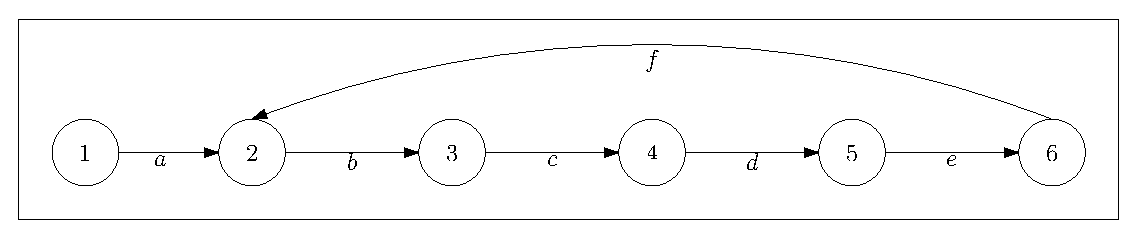
\includegraphics[scale=0.4]{Images/example_network.eps}		\\
	\end{figure}
	%\vspace{1mm}
	\begin{defi}[Incidence Matrix{\footnotemark[1]}]
		The incidence matrix for an oriented graph is defined such that $E(\mathcal{G})_{ij}=+1$ if edge $e_j$ is outgoing from vertex $i$, and $E(\mathcal{G})_{ij}=-1$ if edge $e_j$ is incoming at vertex $i$ and $E(\mathcal{G})_{ij}=0$ otherwise.
	\end{defi}
	%	\pause
	%\begin{block}{Incidence Matrix}
	\vspace{1mm}
	$$E=\begin{bsmallmatrix}
		1 &  0 &  0 &  0 &  0 & \color{cyan}{0} \\
		-1 &  1 &  0 &  0 &  0 & \color{cyan}{-1} \\
		0 & -1 &  1 &  0 &  0 & \color{cyan}{0} \\
		0 &  0 & -1 &  1 &  0 & \color{cyan}{0} \\
		0 &  0 &  0 & -1 &  1 & \color{cyan}{0} \\
		0 &  0 &  0 &  0 & -1 & \color{cyan}{1} \\
	\end{bsmallmatrix}=\begin{bmatrix}\etree & \color{cyan}{E_c}\end{bmatrix}=\etree \begin{bmatrix} I & \color{cyan} T \end{bmatrix}=\etree R$$ 
	where $T=\begin{bmatrix}0 & -1 & -1 & -1 & -1 \end{bmatrix}^T$ and
	$T=(\etree^T\etree)^{-1}\etree^TE_c$
	\\
	\footnotetext[1]{D. Zelazo, Amirreza Rahmani and Mehran Mesbahi, "Agreement via the edge laplacian," 2007 46th IEEE Conference on Decision and Control, New Orleans, LA, USA, 2007, pp. 2309-2314.}
\end{frame}
\begin{frame}
		\begin{defi}[Edge Laplacian of a graph]
		The edge Laplacian for an undirected graph is defined as:  $$\mathcal{L}_{e}:= E^TE,~~~~\letree:= E_\tau^T \etree$$
		where $\mathcal{L}_{e} \in \R^{e \times e}$, $\letree \in \R^{(n-1) \times (n-1)}$
	\end{defi}
			\begin{lemma}[Separation of zero eigenvalue{\footnotemark[1]}]
				Node Laplacian $\mathcal{L}_{n}=EE^T$ for a connected graph $\mathcal{G}$ is similar to $\begin{bmatrix}
					\letree {R}R^T & \textbf{0} \\
					\textbf{0} & 0
				\end{bmatrix}$
			\end{lemma}	
			Proof Outline: Define $S_v=\begin{bmatrix}
				\etree(E_{\tau}^T\etree)^{-1} & \mathbf{1}
			\end{bmatrix}$, thus, $S_v^{-1}=\begin{bmatrix}
				E_{\tau}^T & (1/n)\mathbf{1}^T \end{bmatrix}^T$. Apply the transformation $S_v^{-1}\mathcal{L}_{n}S_v$.					
	\begin{alertblock}{}
		\begin{itemize}
			\item $\letree {R}R^T$ is known as essential edge Laplacian.
			\item Although $\letree$ and $RR^T$ are symmetric matrices, essential edge Laplacian is an asymmetric matrix.
		\end{itemize}
	\end{alertblock}
		\footnotetext[1]{D. Zelazo, Amirreza Rahmani and Mehran Mesbahi, "Agreement via the edge laplacian," 2007 46th IEEE Conference on Decision and Control, New Orleans, LA, USA, 2007, pp. 2309-2314.}
\end{frame}
%%%%%%%%%%%%%%%%%%%%%%%%%%%%%%%%%%%%%%%%%%%%%%%%%%%%

\begin{frame}
	%Transforming the node states to edge states:\\
	%$\dot{X}_e=\begin{bmatrix}
		%	0 & I\\
		%	-E^TE_{in} & -\gamma E^TE_{in}
		%\end{bmatrix}X_e+\begin{bmatrix}
		%	0 & 0\\
		%	E^T & -E^TE_{in} 
		%\end{bmatrix}N(t)$\\
		%where,\\
		%$X=\begin{bmatrix}
			%	x(t) & v(t)
			%\end{bmatrix}^T,X_e=\begin{bmatrix}
			%	x_e(t) & v_e(t)
			%\end{bmatrix}^T,$\\
			%$N=\begin{bmatrix}
				%	q(t) & r(t)
				%\end{bmatrix}^T$,
				%$q(t) \in \R^{n},~~r(t) \in \R^{|e|}$\\
					\begin{lemma}[Coordinate Transformation]
					Using $S_v=\begin{bmatrix}
						\etree(E_{\tau}^T\etree)^{-1} & \mathbf{1}
					\end{bmatrix}$ and applying the coordinate transformation $\begin{bmatrix} S_v & \mathbf{0} \\ \mathbf{0} & S_v \end{bmatrix}\begin{bmatrix} x_e \\ v_e \end{bmatrix}=\begin{bmatrix} x \\ v \end{bmatrix}$, Node states are transformed to new states $x^T_e=\begin{bmatrix*} x^T_{\tau} & x^T_{\mathbf{1}}\end{bmatrix*}^T$, and $v^T_e=\begin{bmatrix*} v^T_{\tau} & v^T_{\mathbf{1}}\end{bmatrix*}^T$
					
					where, $x_\tau,v_\tau \in \R^{n-1}$ are relative state information across the spanning trees and $x_{\mathbf{1}}, v_{\mathbf{1}} \in \R$ are mode in the agreement subspace. 
				\end{lemma}	
				\begin{block}{Reduced Order Edge Dynamics}
					 Using the above coordinate transformation and considering ${X}_{e_\tau}=\begin{bmatrix}
					 	x_\tau^T & v_\tau^T \end{bmatrix}^T$, the reduced order system ($\Sigma_{\tau}$) can be represented as:
					$$\dot{X}_{e_\tau}=\begin{bmatrix}
						\mathbf{0} & I_{n-1}\\
						-\letree RR^T & -\gamma\letree RR^T
					\end{bmatrix}X_{e_\tau}+\begin{bmatrix}
						\mathbf{0} & \mathbf{0}\\
						\sigma_{q}E_{\tau}^T & -\sigma_{r}\letree R
					\end{bmatrix}\hat{N}(t)$$
					$$z(t)=X_{e_\tau}$$
					where, ${X}_{e_\tau} \in \R^{2(n-1)},~\hat{N}(t) \in \R^{(n+|e|)} $ is the normalized noise signal.
				\end{block}
			\end{frame}
\begin{frame}{}
	\begin{defi}[$\mathcal{H}_2$ Norm{\footnotemark[1]}]
		Consider a transfer function $G(s)=\left[
		\begin{array}{c|c}
			A & B \\
			\hline
			C & 0
		\end{array}
		\right]$
		with $A$ stable. Then we have $$\norm{G}_2^2=trace(B^*QB)=trace(CPC^*)$$
		where $Q$ and $P$ are observability and controllability gramians that can be obtained from the following Lyapunov equation:
		$$A^*Q+QA+C^*C=0;~~AP+PA^*+BB^*=0 $$
	\end{defi}
	\pause
	\begin{block}{$\mathcal{H}_2$ norm}
		The $\mathcal{H}_2$ Norm of the system $\Sigma_{\tau}$, where, $A=\begin{bmatrix}
			\mathbf{0} & I_{n-1}\\
			-\letree RR^T & -\gamma\letree RR^T
		\end{bmatrix}$, $B=\begin{bmatrix}
			\mathbf{0} & \mathbf{0}\\
			\sigma_{q}E_{\tau}^T & -\sigma_{r}\letree R
		\end{bmatrix}$ and $C=I_{n-1}$ is given by $$\norm{\Sigma_{\tau}}_2^2=trace(P)$$
		where $P$ is the solution to the Lyapunov equation $AP+PA^T+BB^T=0,$
	\end{block}							
	\footnotetext[1]{Zhou, Kemin, and John Comstock Doyle. Essentials of robust control. Vol. 104. Upper Saddle River, NJ: Prentice hall, 1998.}
\end{frame}

%%%%%%%%%%%%%%%%%%%%%%%%%%%%%%%%%%%%%%%%%%%%%%%%%%%%
\begin{comment}
\begin{frame}{$\mathcal{H}_2$ Norm of the System $\Sigma_{\tau}$}
	Let $P=\begin{bmatrix}
		P_1 & P_2\\
		P_2^T & P_3
	\end{bmatrix}$, $A_3 = -\letree{R}R^T$, and $QQ^T = \sigma_{r}^2 \letree{R}{R}^T\letree^T + \sigma_{q}^2 \etree^T \etree$, \\
	Thus, the Lyapunov equation reduces to the following set of equations:
	\begin{equation*}
		P_2^T = -P_2
	\end{equation*}
	\begin{equation*}
		P_3 + P_1 A_3^T + \gamma P_2 A_3^T = 0
	\end{equation*}
	\begin{equation*}
		P_3 + A_3 P_1 + \gamma A_3 P_2^T = 0
	\end{equation*}
	\begin{equation*}
		A_3 P_2 + P_2^T A_3^T + \gamma A_3 P_3 + \gamma P_3 A_3^T = -QQ^T
	\end{equation*}
	\pause
	Let $\color{blue}J=2\gamma\left[2\gamma^2(I_{n-1} \otimes A_3 + A_3 \otimes I_{n-1}) + 2I_{(n-1)^2} - (A_3^{-1} \otimes A_3 + A_3 \otimes A_3^{-1})\right]^{-1}$, then, solving yields:
	$$\color{magenta}\text{vec}(P_3) = J\text{vec}(-QQ^T)$$
	\vspace{-0.2cm}
	$$\color{magenta}\text{vec}(P_1) = \frac{-1}{2}(I_{n-1} \otimes A_3^{-1} + A_3^{-1} \otimes I_{n-1})\text{vec}(P_3)$$
	\vspace{-0.2cm}
	%$$\color{magenta}\text{vec}(P_2) = \frac{1}{2\gamma}(I \otimes A_3^{-1} - A_3^{-1} \otimes I)\text{vec}(P_3)$$
	\pause
	and hence, the $\mathcal{H}_2$ norm of the system is:
	$$\color{cyan}\|\Sigma_{\tau}\|_2^2 = \text{trace}(P) = \text{trace}(P_1) + \text{trace}(P_3)$$
\end{frame}

\end{comment}
%%%%%%%%%%%%%%%%%%%%%%%%%%%%%%%%%%%%%%%%%%%%%%%%%%%%
\begin{frame}{$\mathcal{H}_2$ Norm for Network of Double Integrators}
	\vspace{-0.2cm}
\begin{myblock}{Theorem 1}
	The $\mathcal{H}_2$ Norm of System $\Sigma_{\tau}$ is 
	$$\norm{\Sigma_{\tau}}^2=\frac{1}{2\gamma}\text{ trace}[(I_{n-1}-A_3^{-1})\color{cyan}{(\sigma_r^2I_{n-1}-\sigma_q^2A_3^{-1})\letree}]$$
	where, $A_3 = -\letree{R}R^T$
\end{myblock}
\textbf{Note:} 
\begin{itemize}
	\item A double integrator network always has a poorer performance than a single integrator.
	\item Norm for double integrator depends on choice of spanning trees unlike single integrator.
\end{itemize}
	\begin{block}{Some Important Properties}
	For an undirected path graph: ($E=\begin{bmatrix}\etree & \color{cyan}{E_c}\end{bmatrix}=\etree \begin{bmatrix} I & \color{cyan} T \end{bmatrix}=\etree R$)
	\begin{itemize}
		\item $\text{trace}[\letree]=2(n-1)$ (True for any spanning tree)
		\item $\text{trace}[\letree^{-1}]=(n-1)(n+1)/6$
		%\item $(RR^T)^{-1}=(I+TT^T)^{-1}$ 
	\end{itemize}
\end{block}
\end{frame}
%%%%%%%%%%%%%%%%%%%%%%%%%%%%%%%%%%%%%%%%%%%%%%%%%%%%
\begin{frame}
	For a path graph with one cycle:
	\begin{itemize}
		\item $(RR^T)^{-1}=(I+TT^T)^{-1}=(I-TT^T/(\ell+1))$ (Matrix Inversion Lemma)
		\item $\text{ trace}[(RR^T)^{-1}]=n-2+1/(\ell+1)]$
		\item $\text{ trace}[(RR^T)^{-1}\letree^{-1}(RR^T)^{-1}]=\text{ trace}[\letree^{-1}-TT^T\letree^{-1}/(\ell+1)]$
	\end{itemize}
\vspace{-0.2cm}
\begin{myblock}{Theorem 2}
		Given an undirected path graph with $n$ node and presence of a cycle of length $\ell$, the $\mathcal{H}_2$ Norm of System $\Sigma_{\tau}$ is
		\vspace{-0.3cm}
		$$\norm{\Sigma_{\tau}}^2=\frac{1}{2\gamma}\left[\textcolor{violet}{2\sigma_r^2(n-1)}+\textcolor{magenta}{(\sigma_{q}^2+\sigma_r^2)(n-2+\frac{1}{\ell+1})}+\textcolor{cyan}{\sigma_q^2\text{ trace}[(RR^T)^{-1}\letree^{-1}(RR^T)^{-1}]}\right]$$
		$$\norm{\Sigma_{\tau}}^2=\frac{1}{2\gamma}\left[\textcolor{violet}{2\sigma_r^2(n-1)}+\textcolor{magenta}{(\sigma_{q}^2+\sigma_r^2)(n-2+\frac{1}{\ell+1})}+\textcolor{cyan}{\sigma_q^2\frac{(n-1)(n+1)}{6}-\sigma_q^2\text{ trace}[\frac{TT^T\letree^{-1}}{\ell+1}]}\right]$$
		where, $\ell=|j-i|$ is the length of cycle and $j,i$ are the end nodes of the edge forming the cycle.
	\end{myblock}
	\vspace{-0.3cm}
	\begin{alertblock}{}
		%$\mathcal{H}_2$ performance is:
		\begin{itemize}
			\item Larger cycle are better.
			\item Increased values of $\gamma$ leads to improvement in performance.
			\item Smaller network performs better than large networks.
		\end{itemize}
	\end{alertblock}
\end{frame}
%%%%%%%%%%%%%%%%%%%%%%%%%%%%%%%%%%%%%%%%%%%%%%%%%%%%
%%%%%%%%%%%%%%%%%%%%%%%%%%%%%%%%%%%%%%%%%%%%%%%%%%%%
\begin{frame}{$\mathcal{H}_2$ Norm of the system with varying cycle length in a network}
	%\vspace{-0.5cm}
	\begin{figure}
		%\hspace{-1cm}
		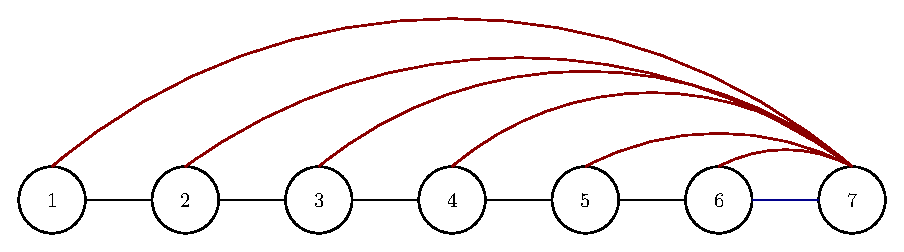
\includegraphics[scale=0.5]{Images/one_cycle_undirected.eps}
	\end{figure}
			%\vspace{-0.7cm}
			\begin{figure}
				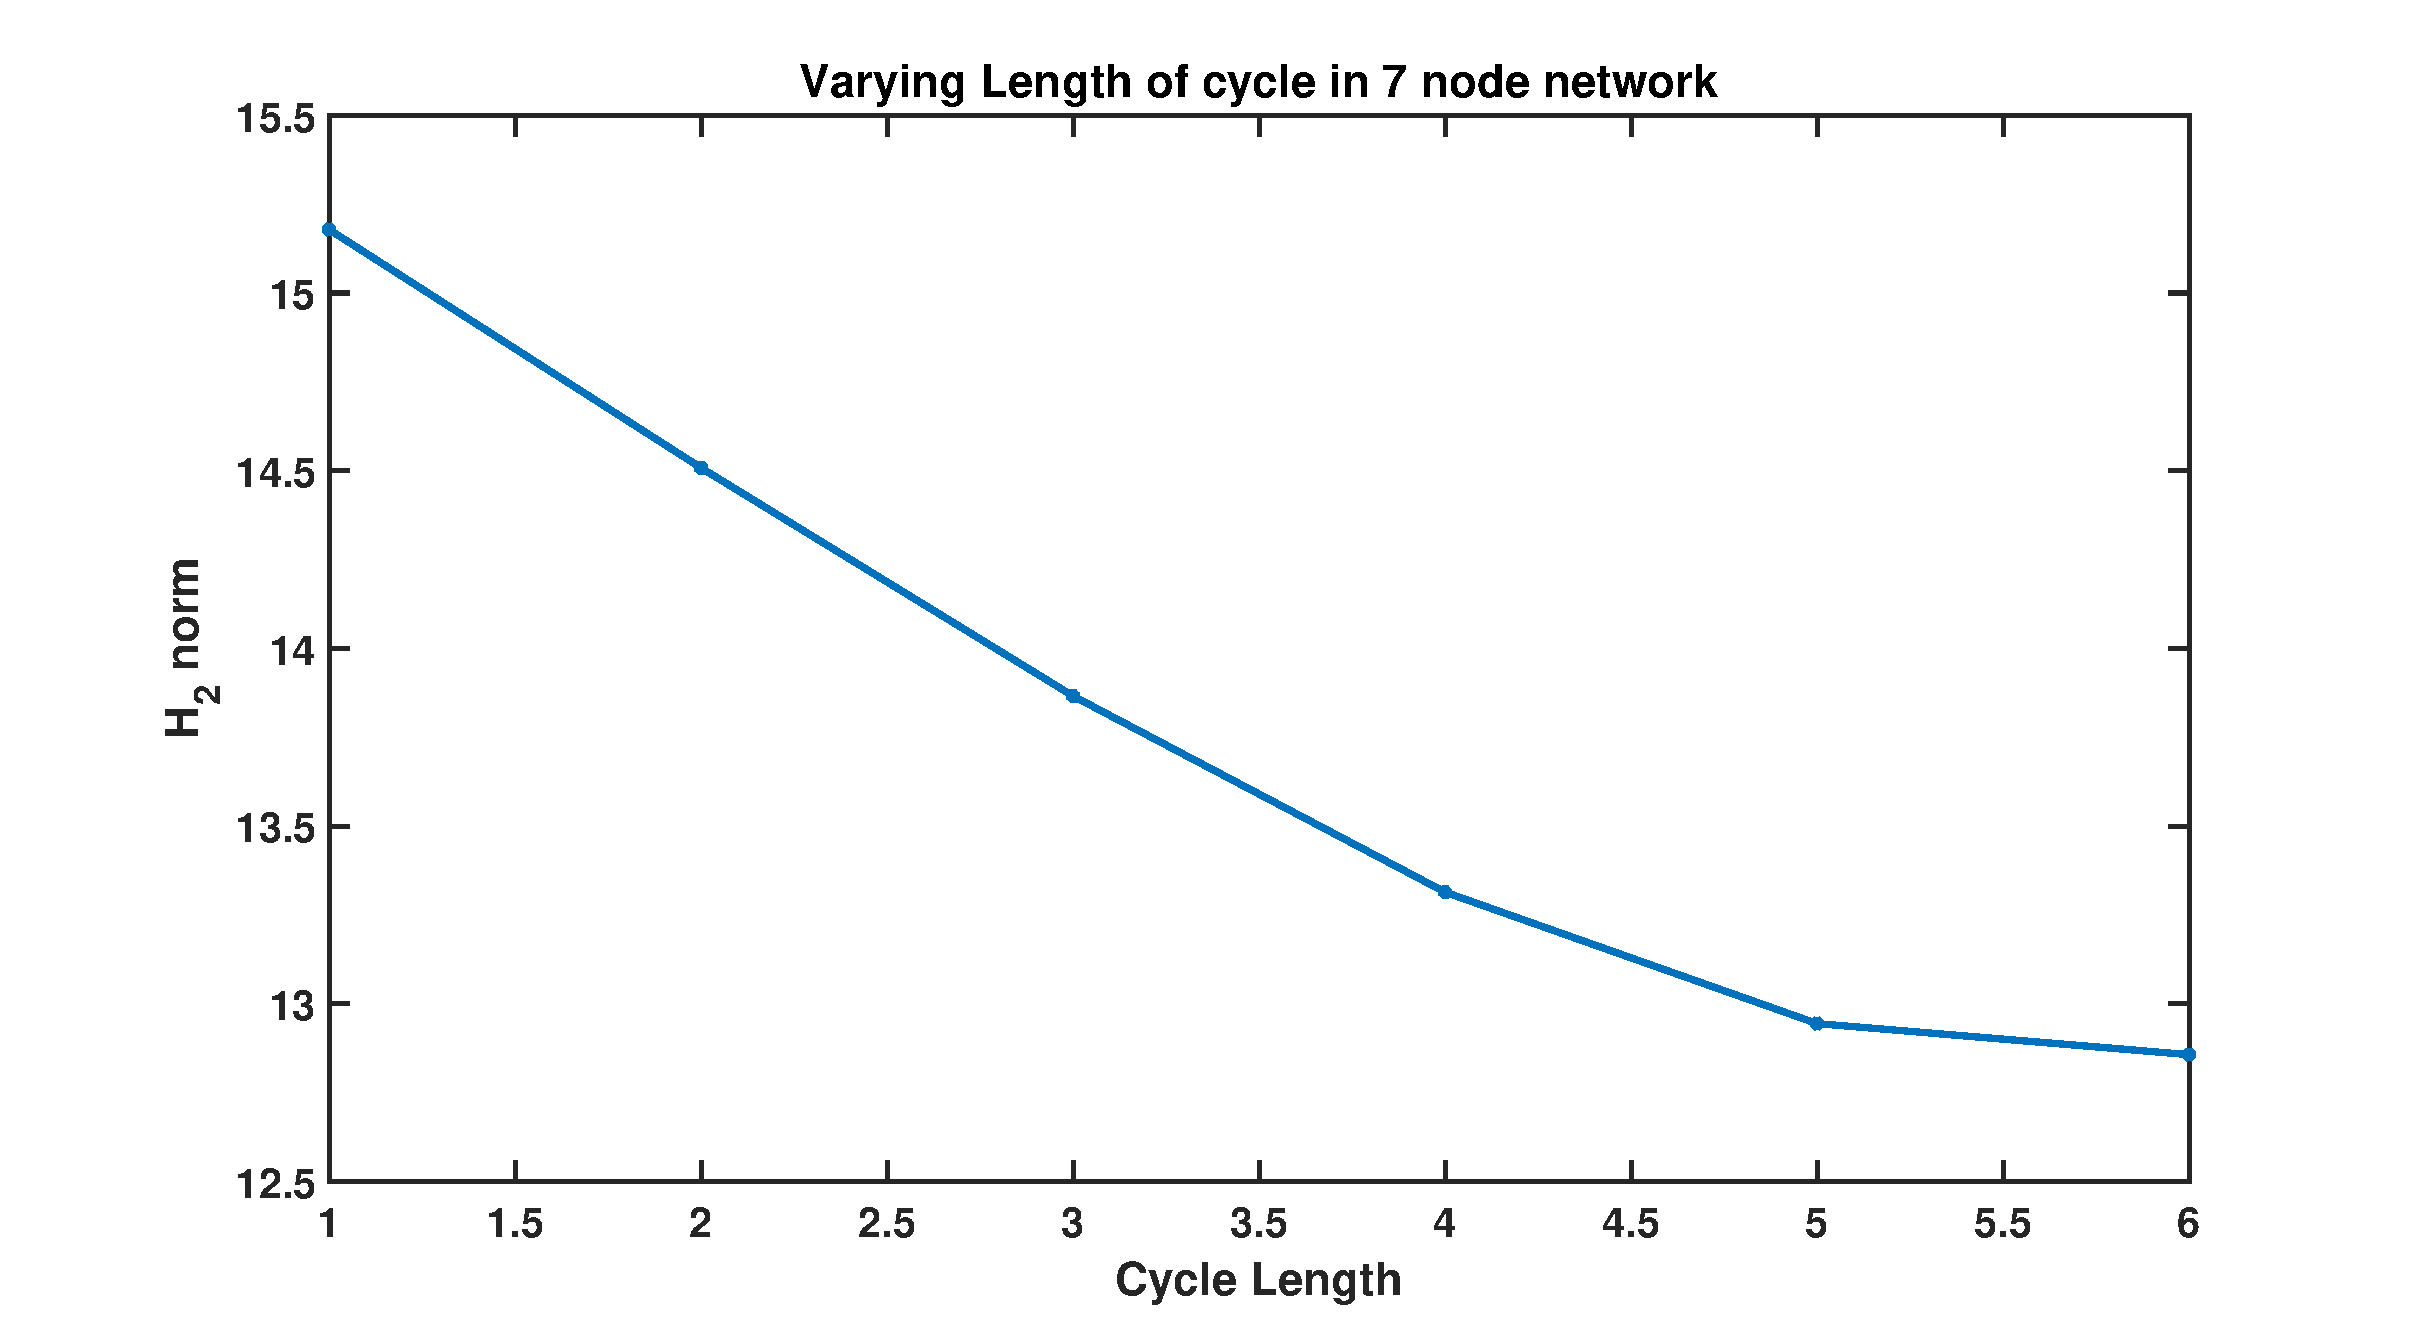
\includegraphics[scale=0.2]{Images/Single_Cycle_Varying_Length.eps}
			\end{figure}
\end{frame}
%%%%%%%%%%%%%%%%%%%%%%%%%%%%%%%%%%%%%%%%%%%%%%%%%%%%
\begin{frame}
		\begin{myblock}{Theorem 3}
		Given an undirected path graph on $n$ double integrators, addition of an edge that leads to the formation of a cycle of length $\ell < n $, results in $\mathcal{H}_2$ norm of a system $\Sigma_{\tau}$ is given by:
		$$\norm{\Sigma_{\tau}}^2=\frac{1}{2\gamma}\left[\textcolor{violet}{2\sigma_r^2(n-1)}+\textcolor{magenta}{(\sigma_{q}^2+\sigma_r^2)(n-2+\frac{1}{\ell+1})}+\textcolor{cyan}{\sigma_q^2\frac{(n-1)(n+1)}{6}-\frac{\sigma_q^2(\ell+2)}{(\ell+1)^2}\text{ trace}[TT^T\letree^{-1}]}\right]$$
	\end{myblock}
\vspace{-0.3cm}
\begin{alertblock}{}
	\begin{itemize}
\item For a cycle of length $\ell, ~~\text{trace}[TT^T\letree^{-1}]$ is maximum if the cycle is at the center of the tree.	
\end{itemize}
\end{alertblock}
\vspace{-0.5cm}
	$$TT^T=\begin{bmatrix}
		0 & 0 & 0 & 0 & 0 & 0 \\
		0 & 1 & 1 & 0 & 0 & 0 \\
		0 & 1 & 1 & 0 & 0 & 0 \\
		0 & 0 & 0 & 0 & 0 & 0 \\
		0 & 0 & 0 & 0 & 0 & 0 \\
		0 & 0 & 0 & 0 & 0 & 0 
	\end{bmatrix},~~\letree^{-1}=\begin{bmatrix}
	0.8571 & 0.7143 & 0.5714 & 0.4286 & 0.2857 & 0.1429 \\
	0.7143 & 1.4286 & 1.1429 & 0.8571 & 0.5714 & 0.2857 \\
	0.5714 & 1.1429 & 1.7143 & 1.2857 & 0.8571 & 0.4286 \\
	0.4286 & 0.8571 & 1.2857 & 1.7143 & 1.1429 & 0.5714 \\
	0.2857 & 0.5714 & 0.8571 & 1.1429 & 1.4286 & 0.7143 \\
	0.1429 & 0.2857 & 0.4286 & 0.5714 & 0.7143 & 0.8571 
	\end{bmatrix}$$
	$$\text{trace}[TT^T\letree^{-1}]=5.4286$$
\end{frame}
%%%%%%%%%%%%%%%%%%%%%%%%%%%%%%%%%%%%%%%%%%%%%%%%%%%%
\begin{frame}{$\mathcal{H}_2$ Norm of the system with cycle length in presence of single cycle}
	%\vspace{-0.5cm}
		\begin{figure}
		%\hspace{-1cm}
		\includegraphics[scale=0.5]{Images/same_length2_different_position_undirected.eps}
	\end{figure}
	\begin{columns}
		\begin{column}{0.5\textwidth}
			%\vspace{-0.7cm}
			\begin{figure}
				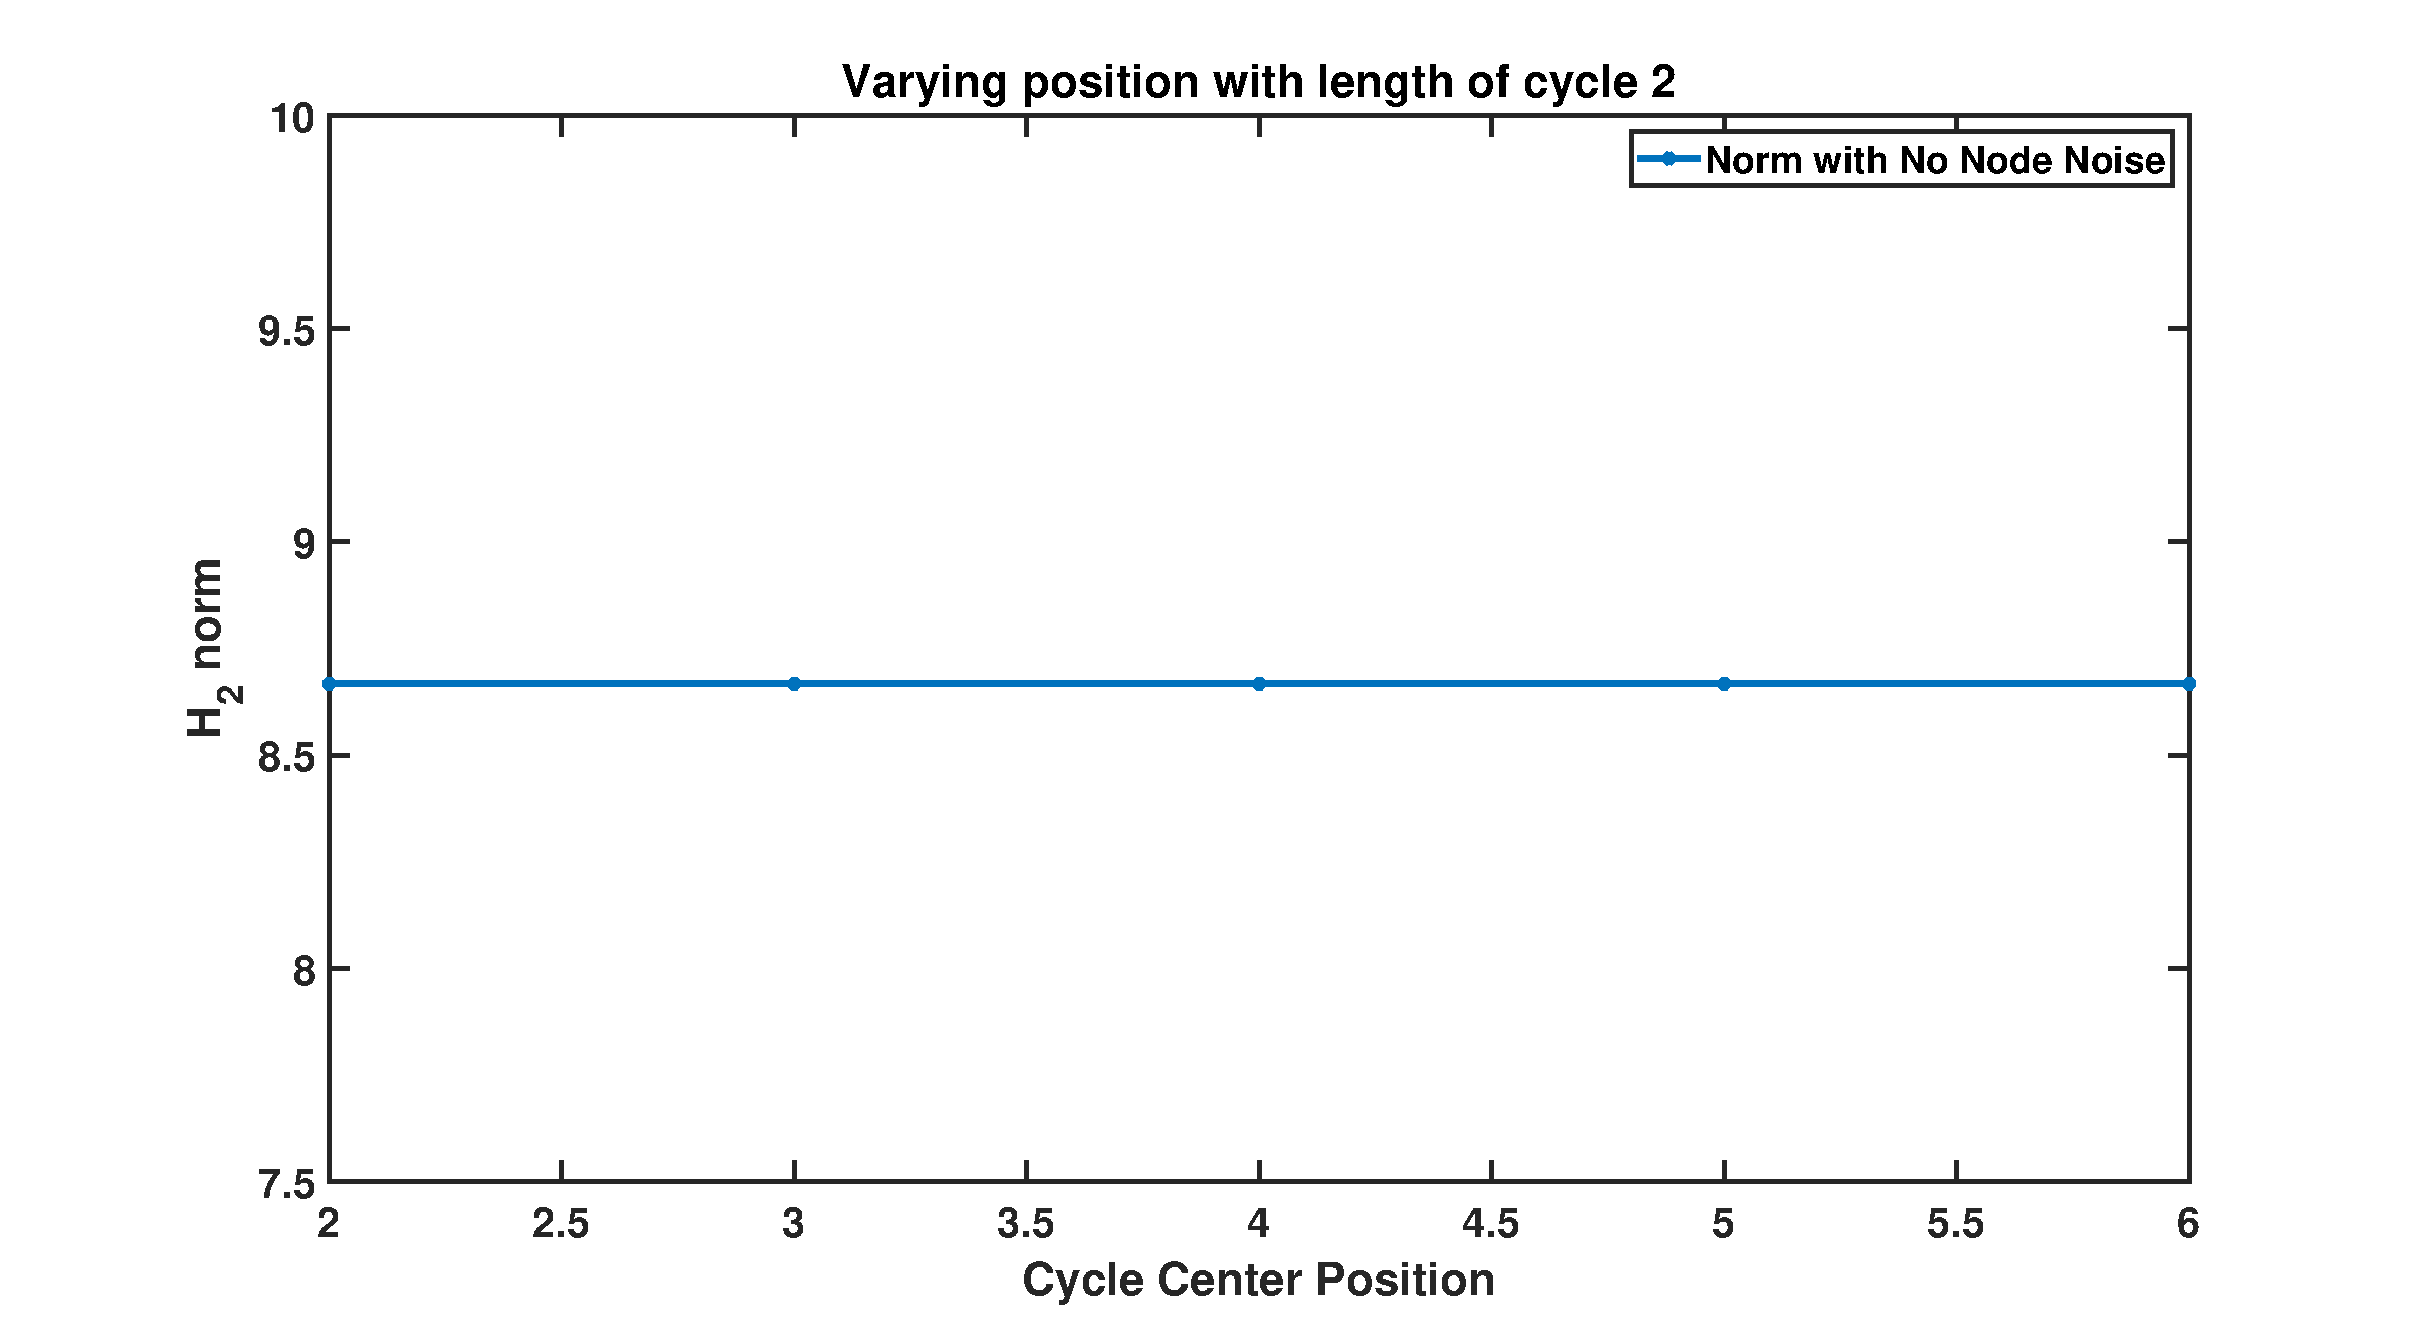
\includegraphics[scale=0.2]{Images/Single_Cycle_Length2_unidrected_Absent_Node_Noise.eps}
			\end{figure}
		\end{column}
		\begin{column}{0.5\textwidth}
			%\vspace{-0.7cm}
		\begin{figure}
				\centering
				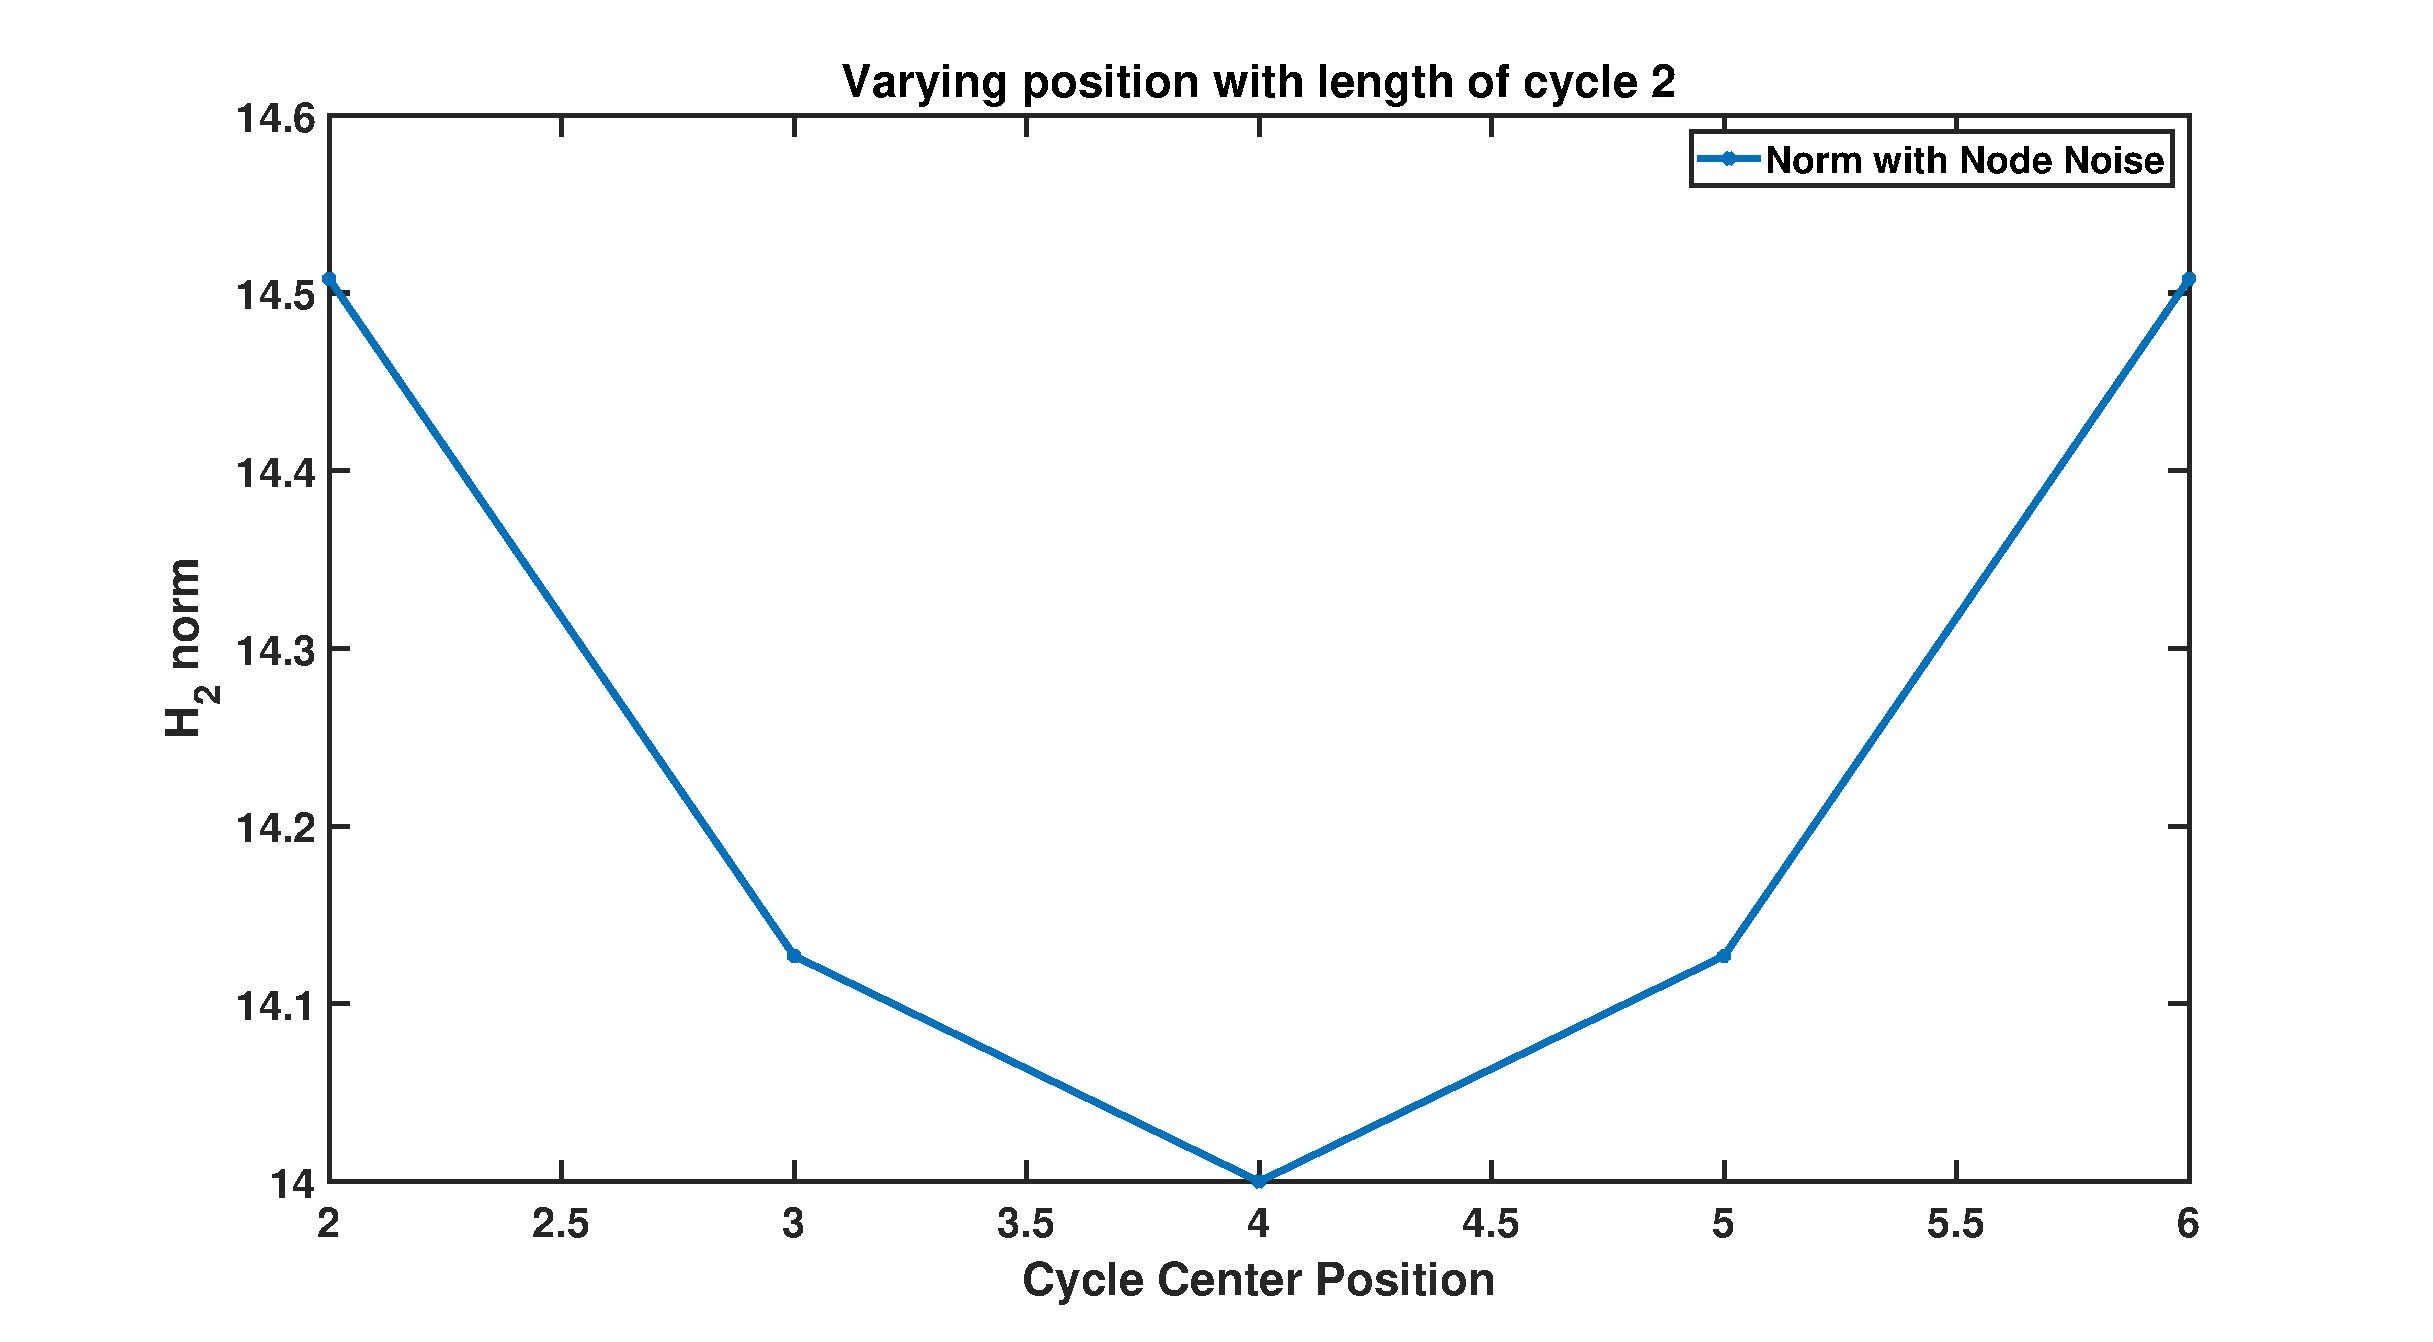
\includegraphics[scale=0.2]{Images/Single_Cycle_Length2_unidrected_Present_Node_Noise.eps}
			\end{figure}
		\end{column}
	\end{columns}
	\vspace{-0.2cm}	
\end{frame}
%%%%%%%%%%%%%%%%%%%%%%%%%%%%%%%%%%%%%%%%%%%%%%%%%%%%

\begin{frame}{Path Graph with Single Cycle}
	\begin{alertblock}{Conclusion}
		\begin{itemize}[]
			\item Performance improves with increase in the value of $\gamma$.
			\item Performance degrades with increase in the network size i.e with increase in $n$.
			\item The performance improves with increase in length of the cycle $\ell$. Hence larger cycles are better. 
			\item If the node noise is zero, then the position of cycle does not impact the performance. Hence, in presence of edge noise only, the size of cycle is enough to characterize the performance. 
			\item However, in presence of node noise with single cycle, the performance depends also on the location of the cycle.
			\item Thus, among two cycles of same size, the cycle towards center of the tree gives better performance. 
		\end{itemize}
	\end{alertblock}
\end{frame}
%%%%%%%%%%%%%%%%%%%%%%%%%%%%%%%%%%%%%%%%%%%%%%%%%%%%
\begin{frame}{Two interacting Cycles in Undirected Path graph}
	\begin{figure}
		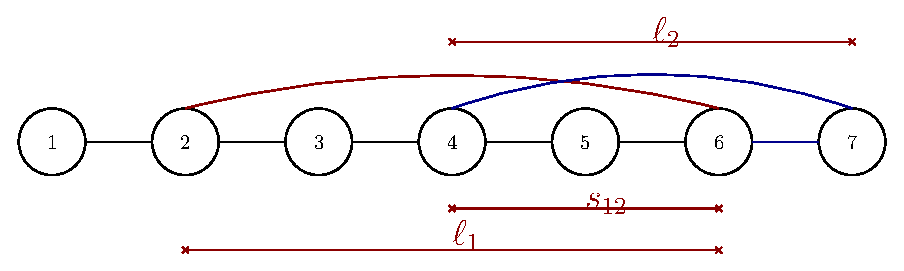
\includegraphics[scale=0.8]{Images/2_InteractingCycles_undirected.eps}
	\end{figure}
	\begin{myblock}{Theorem 4}
		Given an undirected path graph with $n$ node and presence of two cycle of length $\ell_1,\ell_2$ and number of overlapping edges $s_{12}$, then $\mathcal{H}_2$ Norm of System $\Sigma_{\tau}$ is
		
		$$\norm{\Sigma_{\tau}}^2=\frac{1}{2\gamma}\left[\textcolor{violet}{2\sigma_r^2(n-1)}+\textcolor{magenta}{(\sigma_{q}^2+\sigma_r^2)(n-3+D)}+\textcolor{cyan}{\sigma_q^2\text{ trace}[(RR^T)^{-1}\letree^{-1}(RR^T)^{-1}}\right]$$
		
		where $D=\frac{\ell_1+\ell_2+2}{(\ell_1+1)(\ell_2+1)-s_{12}^2}$
		
	\end{myblock}
\end{frame}	
%%%%%%%%%%%%%%%%%%%%%%%%%%%%%%%%%%%%%%%%%%%%%%%%%%%%
\begin{comment}
\begin{frame}{Two interacting Cycles in Undirected Path graph}
	In absence of node noise
	$\norm{\Sigma_{\tau}}^2=\frac{1}{2\gamma}\left[\textcolor{violet}{2\sigma_r^2(n-1)}+\textcolor{magenta}{\sigma_r^2(n-3+D)}\right]$ \\
	Thus, cycle lengths and overlap is enough to characterize performance.
	\begin{figure}
		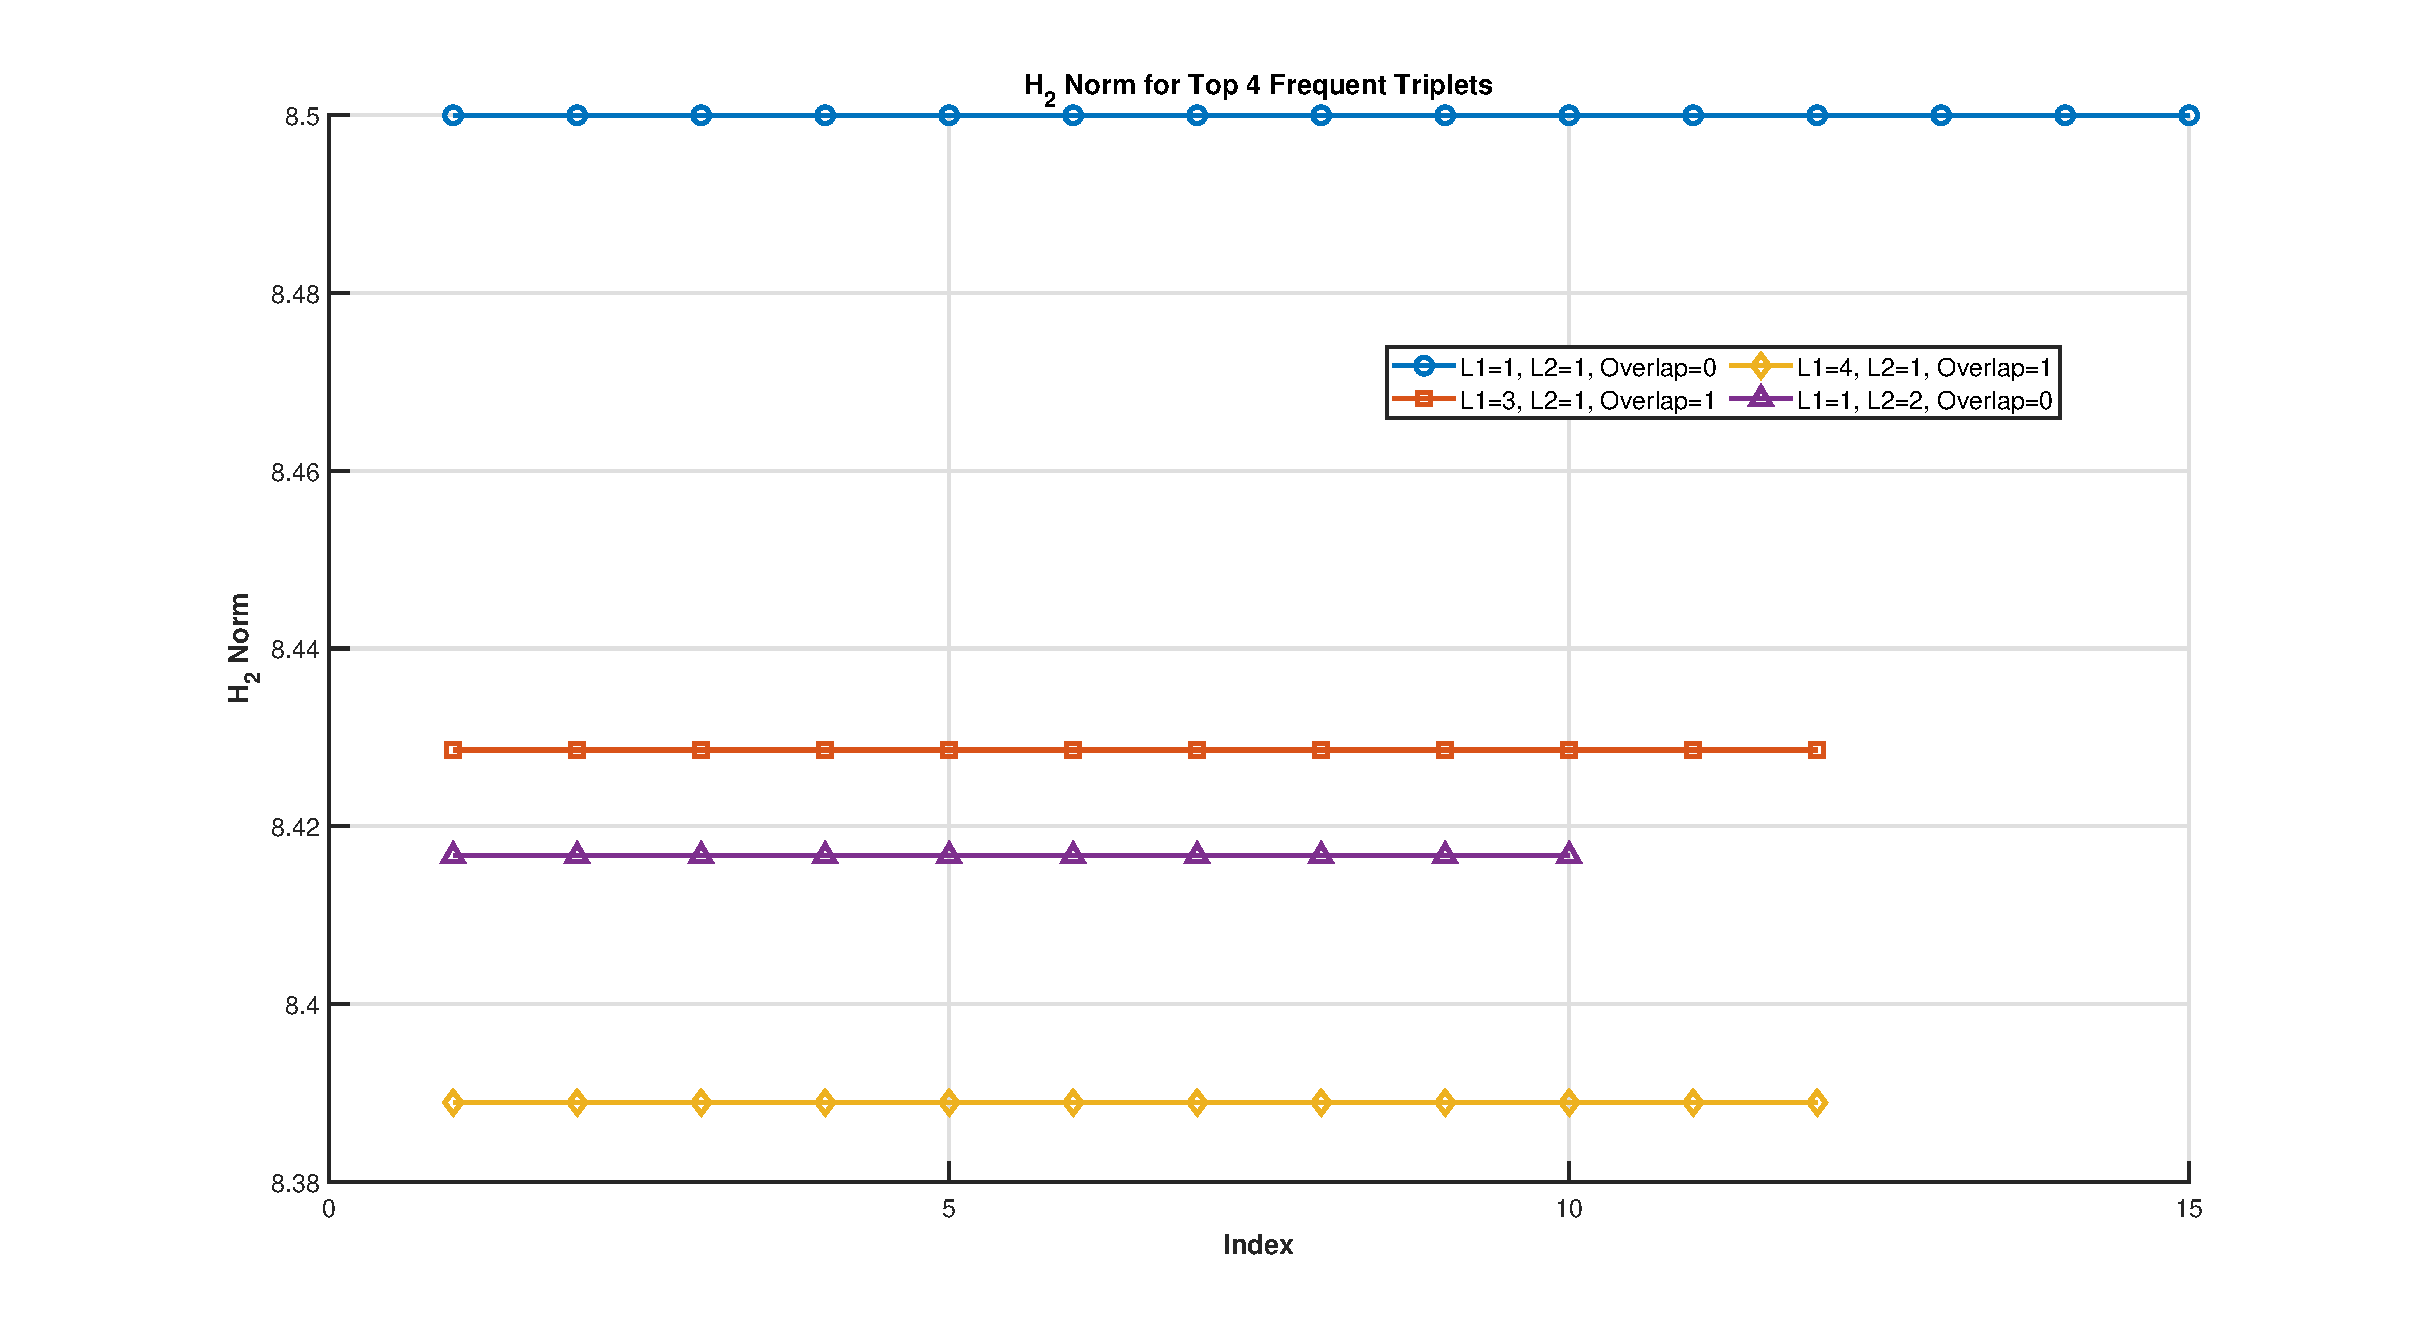
\includegraphics[scale=0.19]{Images/4_most_frequent_triplets.eps}
		\hspace{-0.5cm}
		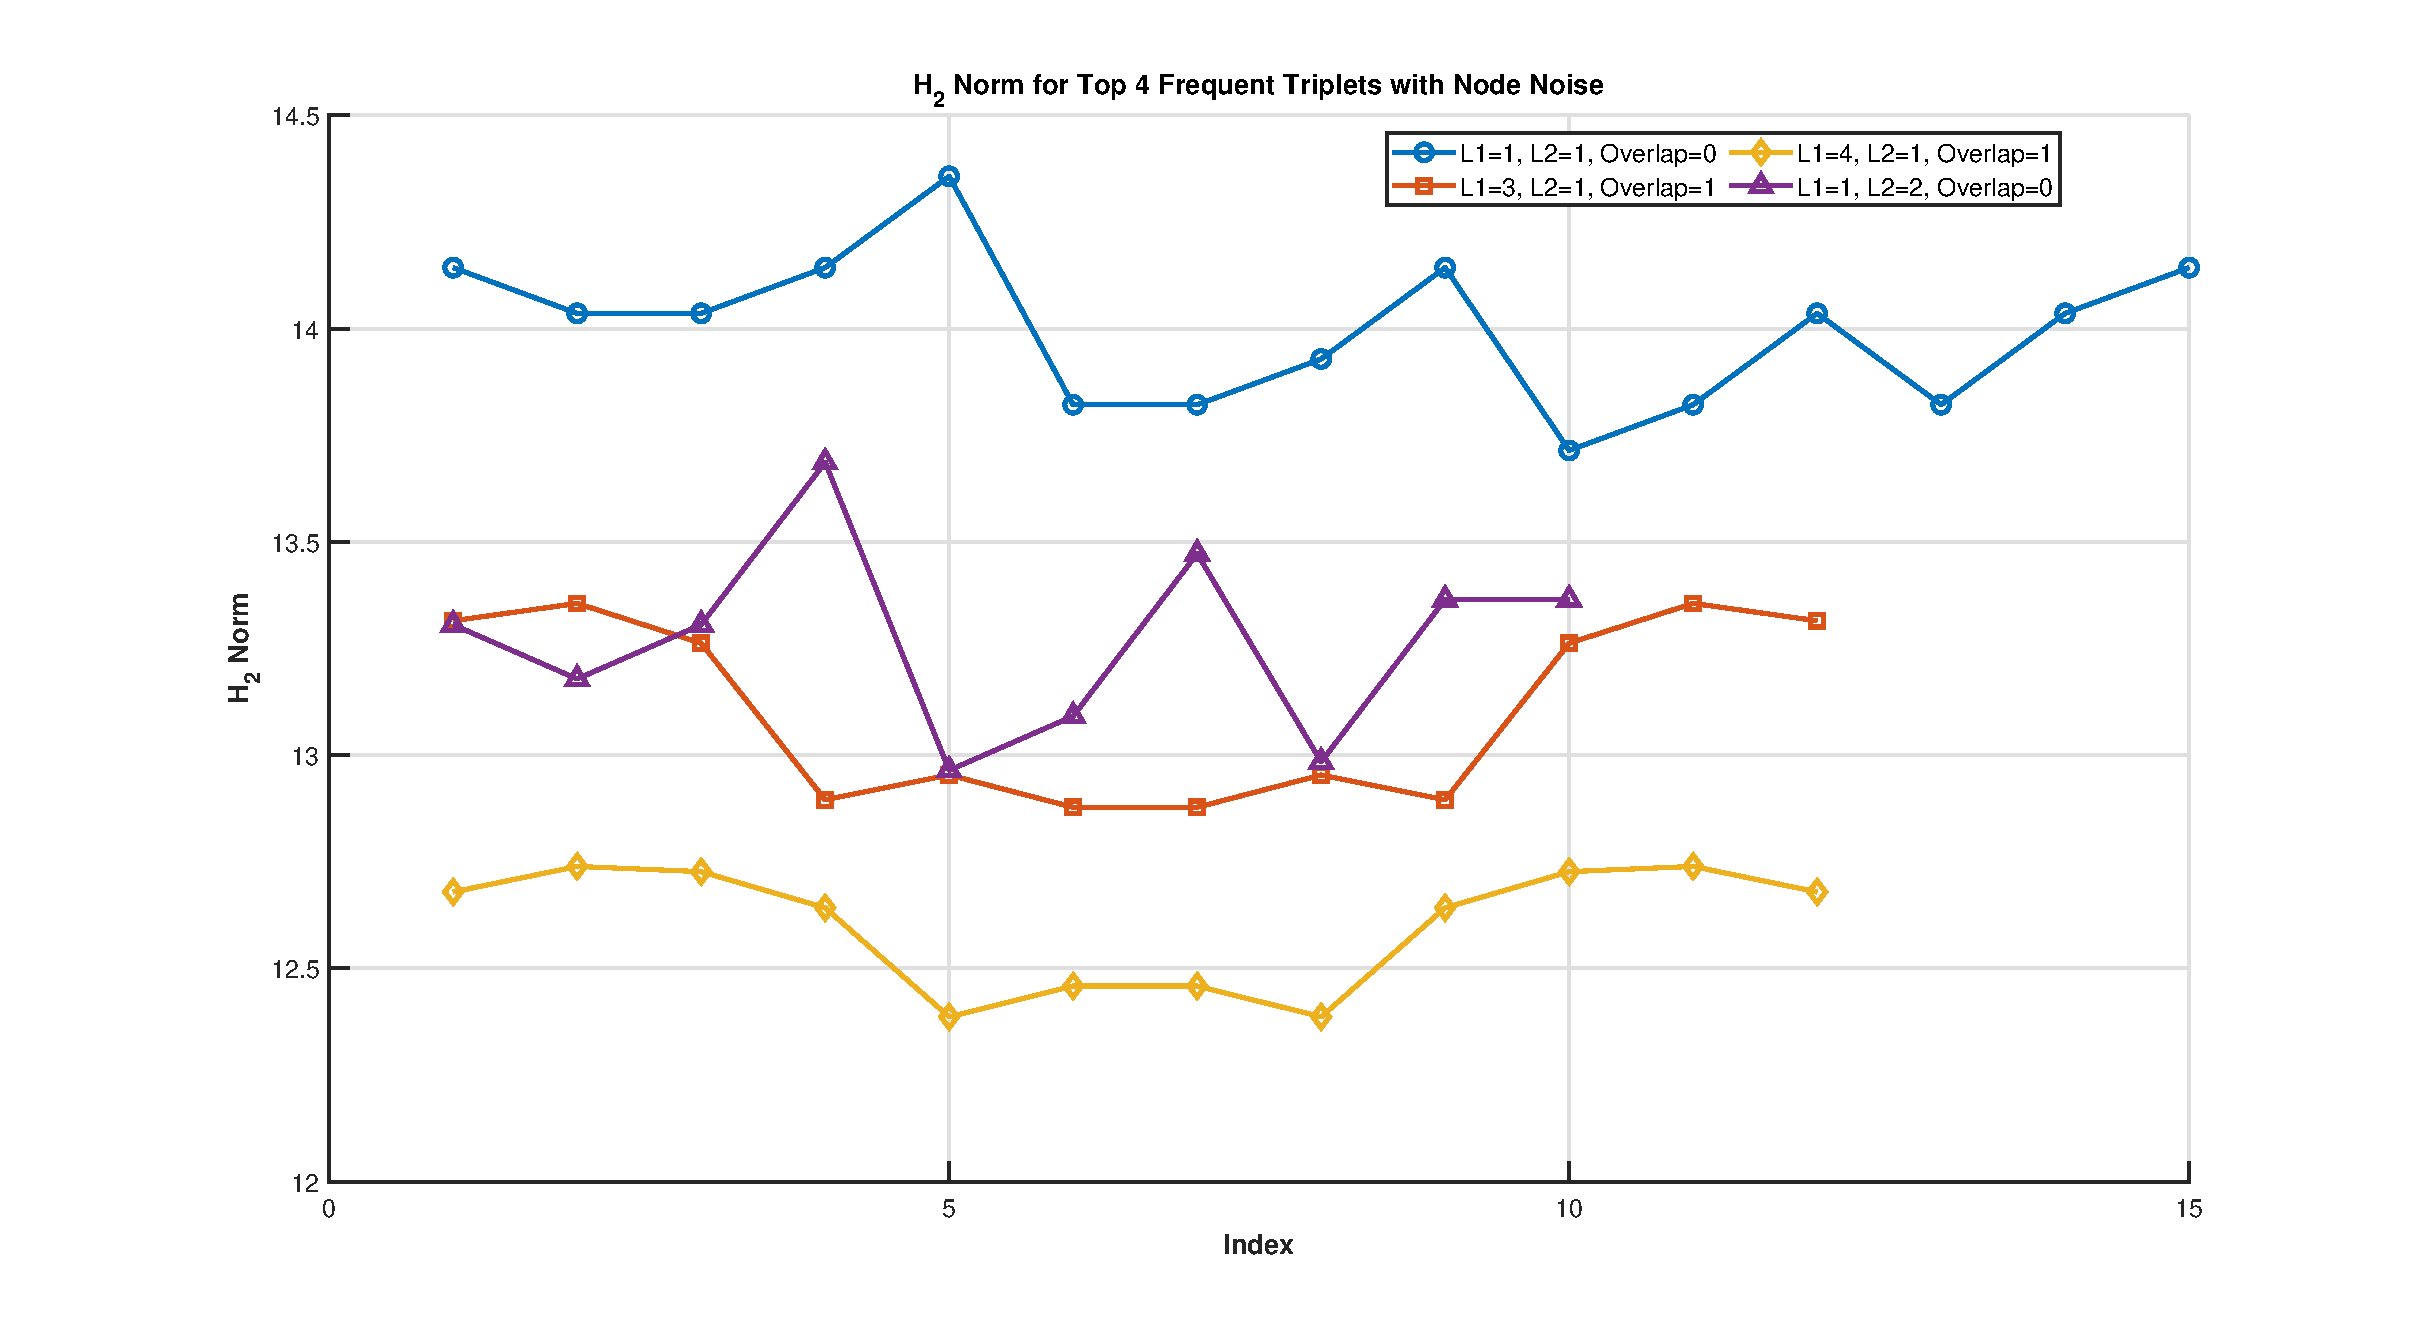
\includegraphics[scale=0.19]{Images/4_most_frequent_triplets_with_node_noise.eps}
	\end{figure}
\end{frame}	
%%%%%%%%%%%%%%%%%%%%%%%%%%%%%%%%%%%%%%%%%%%%%%%%%%%%
\begin{frame}{Two interacting Cycles in Undirected Path graph}
	Lengths Vs $\mathcal{H}_2$ Norm for $n=7$
	\begin{figure}
		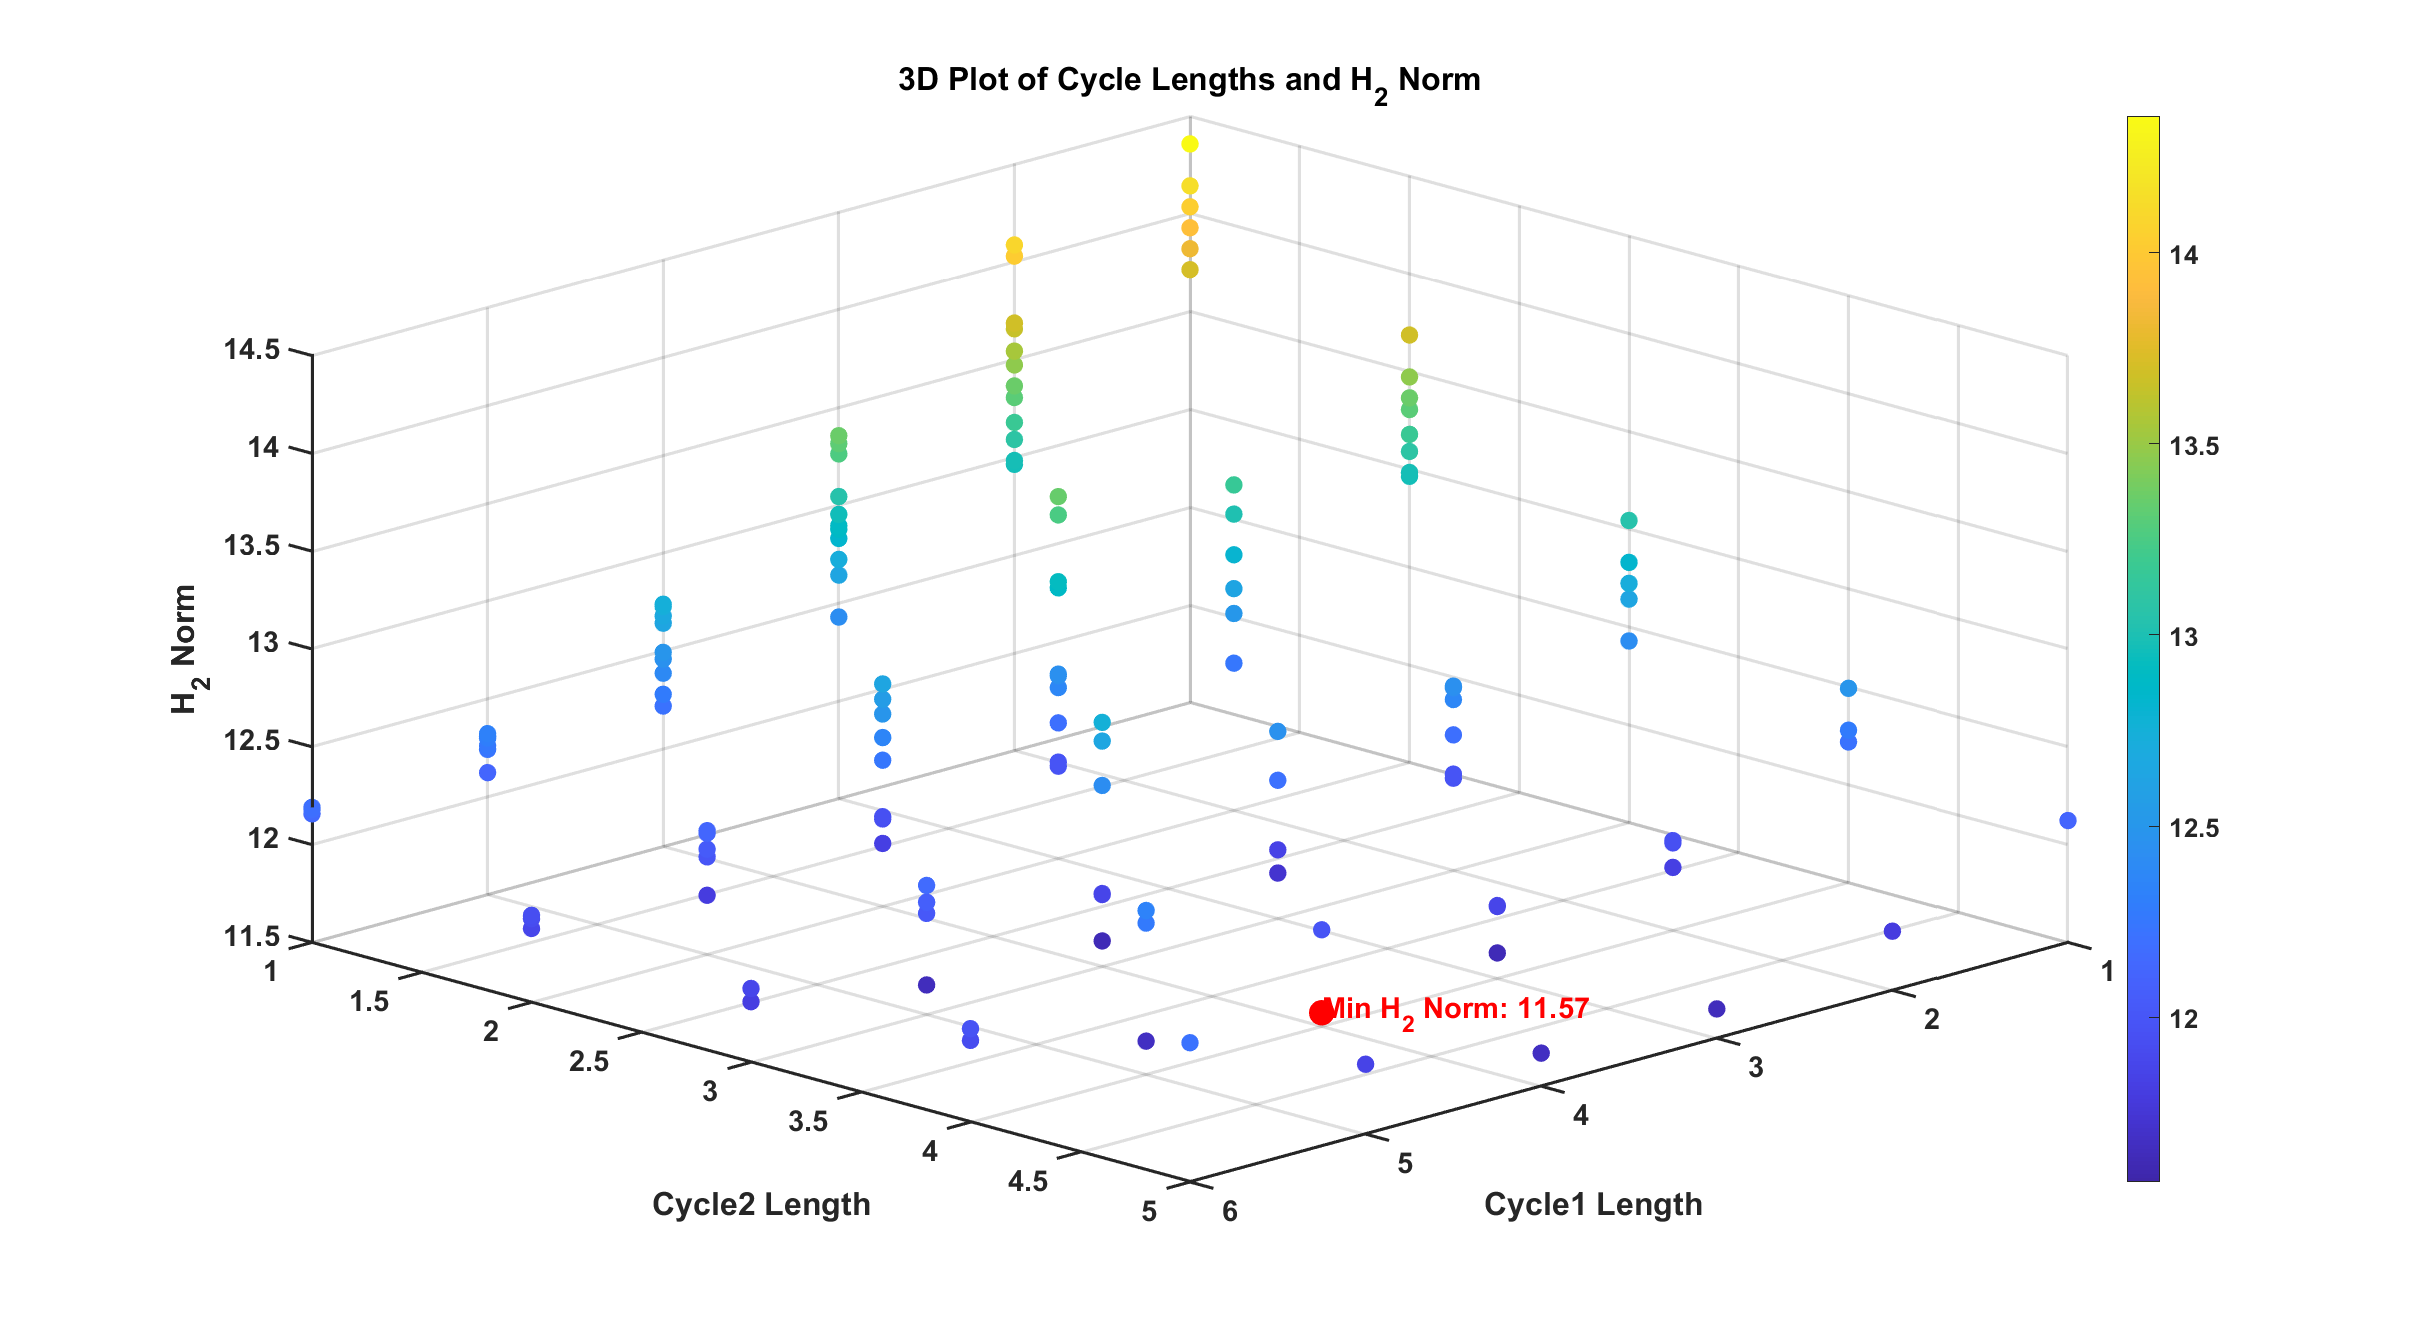
\includegraphics[scale=0.3]{Images/Two_Cycles_Length_Variations_H2_norm.eps}
	\end{figure}
\end{frame}	
%%%%%%%%%%%%%%%%%%%%%%%%%%%%%%%%%%%%%%%%%%%%%%%%%%%%
\begin{frame}{Two interacting Cycles in Undirected Path graph}
	Edge Overlaps Vs $\mathcal{H}_2$ Norm for $n=7$
	\begin{figure}
		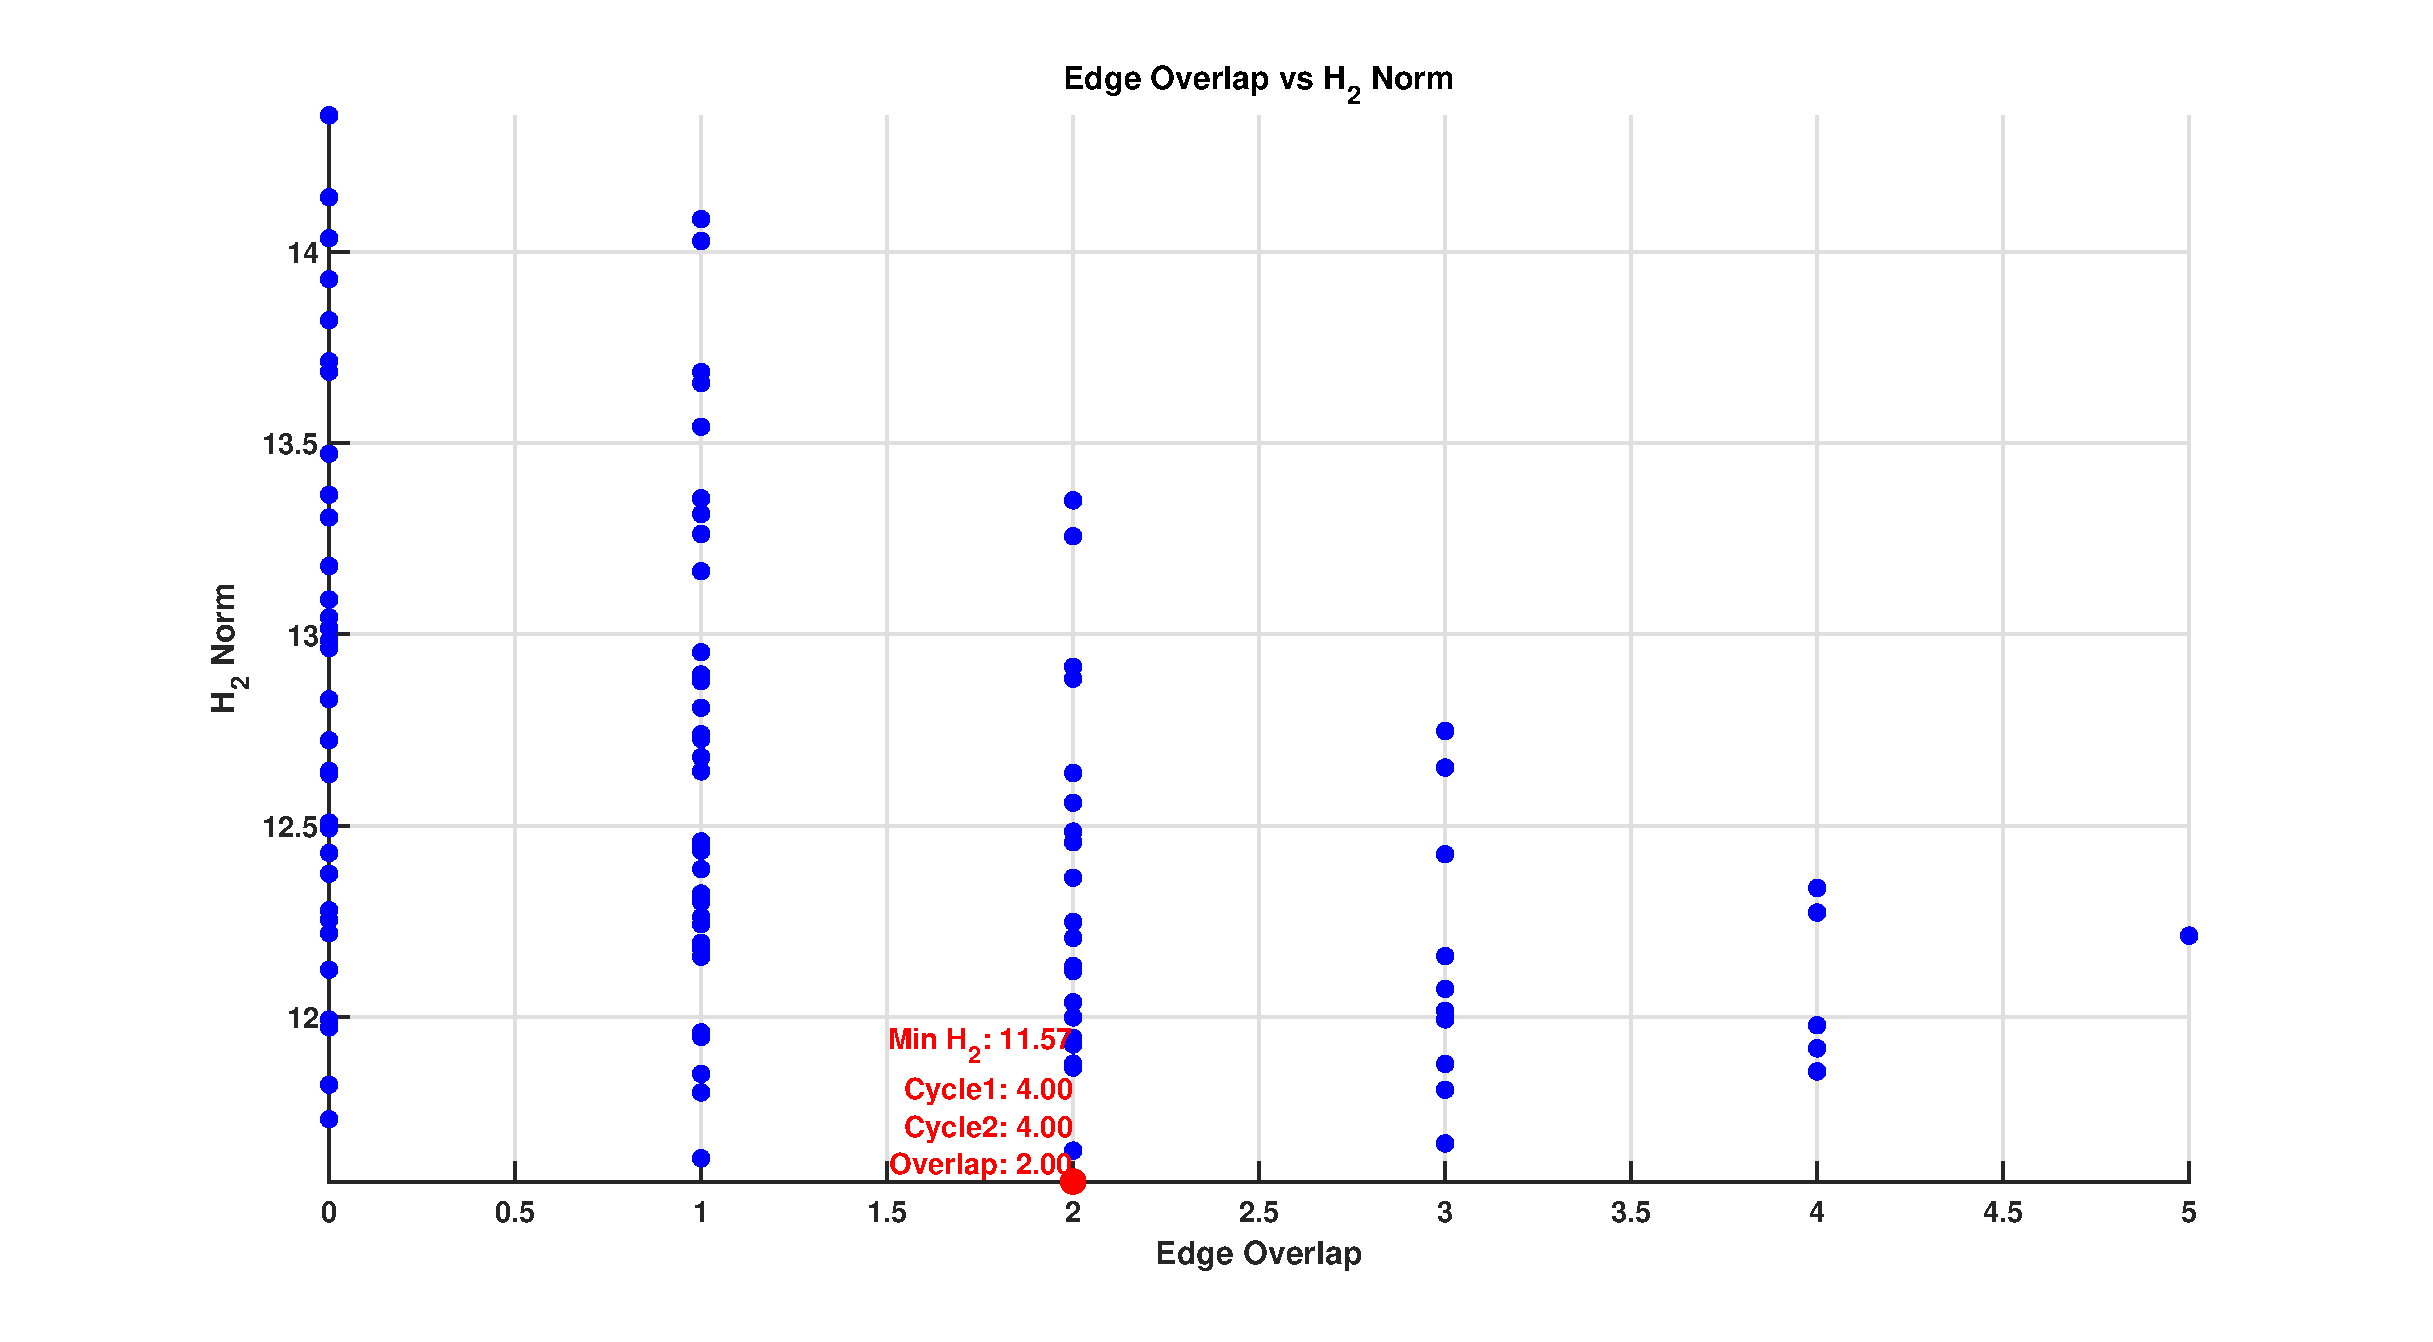
\includegraphics[scale=0.3]{Images/H2_norm_with_edge_overlap.eps}
	\end{figure}
\end{frame}	

\end{comment}
%%%%%%%%%%%%%%%%%%%%%%%%%%%%%%%%%%%%%%%%%%%%%%%%%%%%
\begin{frame}{Path Graph with Two Cycles}
	
	\begin{block}{}
		$\text{Trace}\left[(RR^T)^{-1}\letree^{-1}(RR^T)^{-1}\right]=\text{trace}\left[\letree^{-1}+(\frac{1}{D^2})\letree^{-1}(c_1t_1t_1^T+c_2t_2t_2^T+2c_3t_1t_2^T)\right]$\\
		where, \\
		$t_1,t_2$ are columns of $T$ corresponding to cycles 1 and 2,\\
		$c_1=\ell_1(\ell_2+1)^2-(\ell_2+2)s_{12}^2-2D(\ell_2+1)$\\
		$c_2=\ell_2(\ell_1+1)^2-(\ell_1+2)s_{12}^2-2D(\ell_1+1)$\\
		$c_3=s_{12}(s_{12}^2+2D+1-\ell_1\ell_2)$
		%Given a path graph with $n$ node and two cycle of size $\ell_1, \ell_2$ with $s_{12}$ overlapping edges between the cycles, the $\mathcal{H}_2$ Norm of System $\Sigma_{\tau}$ in presence of node noise depends on the location of cycles and is independent of its location in absence of node noise.
	\end{block}
	\begin{alertblock}{}
	\begin{itemize}
		\item In absence of node noise, the performance only depends on the size of the cycles and the number of overlapping edges but independent of the position of the cycles in the network.
		\item The best performance is achieved with near equal sized cycles ($|\ell_1-\ell_2|\le1$) from two extreme edges of spanning trees.
		\item The number of overlapping edges for best performance increases with the increase in size of network.
	\end{itemize}
\end{alertblock}

\end{frame}
%%%%%%%%%%%%%%%%%%%%%%%%%%%%%%%%%%%%%%%%%%%%%%%%%%%%
\begin{comment}
\begin{frame}{For Directed Path Graph}
	\begin{figure}
		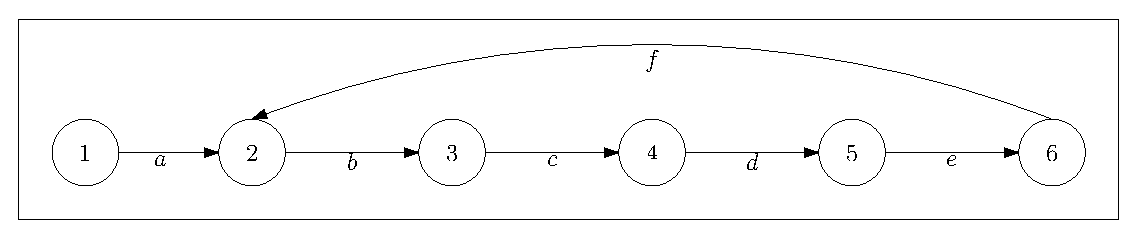
\includegraphics[scale=0.4]{Images/example_network.eps}		\\
	\end{figure}
	\vspace{-0.3cm}
\begin{defi}[In-incidence Matrix{\footnotemark[1]}]
				The In-incidence matrix for a digraph $\mathcal{G}$ is defined such that $E_{in}(\mathcal{G})_{ij}=-1$ if edge $e_j$ is incoming at vertex $i$ and $E(\mathcal{G})_{ij}=0$ otherwise.
\end{defi}
$E_{in}=\begin{bsmallmatrix}
				0 &  0 &  0 &  0 &  0 & \color{cyan}{0} \\
				-1 &  0 &  0 &  0 &  0 & \color{cyan}{-1} \\
				0 & -1 &  0 &  0 &  0 & \color{cyan}{0} \\
				0 &  0 & -1 &  0 &  0 & \color{cyan}{0} \\
				0 &  0 &  0 & -1 &  0 & \color{cyan}{0} \\
				0 &  0 &  0 &  0 & -1 & \color{cyan}{0} \\
\end{bsmallmatrix}$;
			$~~E_{in}=\begin{bmatrix}\etreein & \color{cyan}{E_{c_{in}}}\end{bmatrix}=\etreein \begin{bmatrix} I_{n-1} & \color{cyan}{\tilde{T}}\end{bmatrix}=\etreein \tilde{R}$,\\
			where $\tilde{T}=\begin{bmatrix}1 & 0 & 0 & 0 & 0 \end{bmatrix}^T=(\etreein^T\etreein)^{-1}\etreein^TE_{c_{in}}$\\
\textcolor{red}{Note:} Relation above holds only if graph has a \color{blue}{unique root node}.
	\footnotetext[1]{Mukherjee, Dwaipayan, and Daniel Zelazo. "Robustness of consensus over weighted digraphs." IEEE Transactions on Network Science and Engineering 6.4 (2018): 657-670.}
\end{frame}

%%%%%%%%%%%%%%%%%%%%%%%%%%%%%%%%%%%%%%%%%%%%%%%%%%%%
\begin{frame}
	\begin{block}{Reduced Order Edge Dynamics}
		Applying similar coordinate transformation to separate the zero eigenvalue, the reduced order system ($\Sigma_{\tau}$) can be represented as:
		$$\dot{X}_{e_\tau}=\begin{bmatrix}
			\mathbf{0} & I_{n-1}\\
			-\letreein \tilde{R}R^T & -\gamma\letreein \tilde{R}R^T
		\end{bmatrix}X_{e_\tau}+\begin{bmatrix}
			\mathbf{0} & \mathbf{0}\\
			\sigma_{q}E^T & -\sigma_{r}\letreein \tilde{R}
		\end{bmatrix}\hat{N}(t)$$
		$$z(t)=X_{e_\tau}$$
		where, ${X}_{e_\tau} \in \R^{2(n-1)},~ \hat{N}(t) \in \R^{(n+|e|)} $ is the normalized noise signal.
	\end{block}
	\pause
	\begin{block}{$\mathcal{H}_2$ norm}
		The $\mathcal{H}_2$ Norm of the system $\Sigma_{\tau}$, where, $A=\begin{bmatrix}
			\mathbf{0} & I_{n-1}\\
			-\letreein \tilde{R}R^T & -\gamma\letreein \tilde{R}R^T
		\end{bmatrix}$, $B=\begin{bmatrix}
			\mathbf{0} & \mathbf{0}\\
			\sigma_{q}E^T & -\sigma_{r}\letreein \tilde{R}
		\end{bmatrix}$ and $C=I_{n-1}$ is given by $$\norm{\Sigma_{\tau}}_2^2=trace(P)$$
		where $P$ is the solution to the Lyapunov equation $AP+PA^T+BB^T=0,$
	\end{block}							
\end{frame}


\begin{frame}{$\mathcal{H}_2$ Norm of the system with variation in $\gamma$ }
	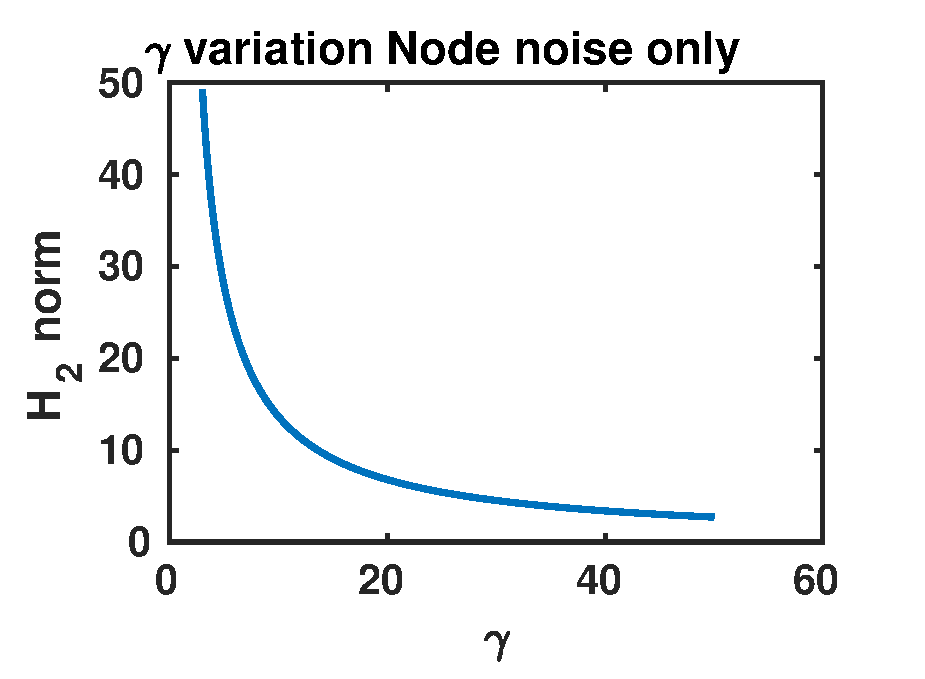
\includegraphics[scale=0.33]{Images/H2normwithgamma_Nodenoise.eps}
	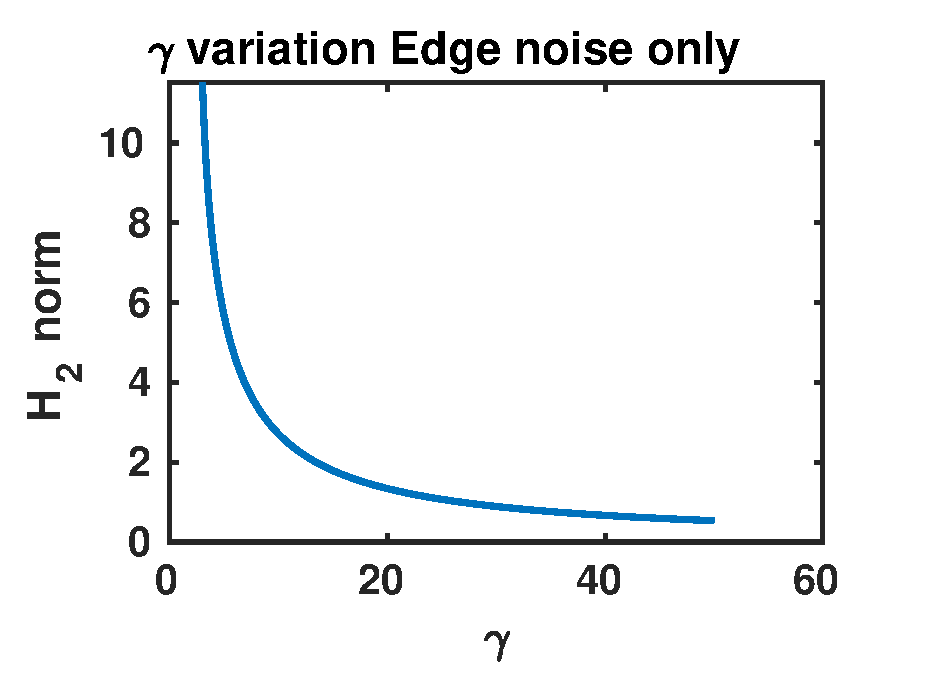
\includegraphics[scale=0.33]{Images/H2normwithgamma_Edgenoise.eps}
	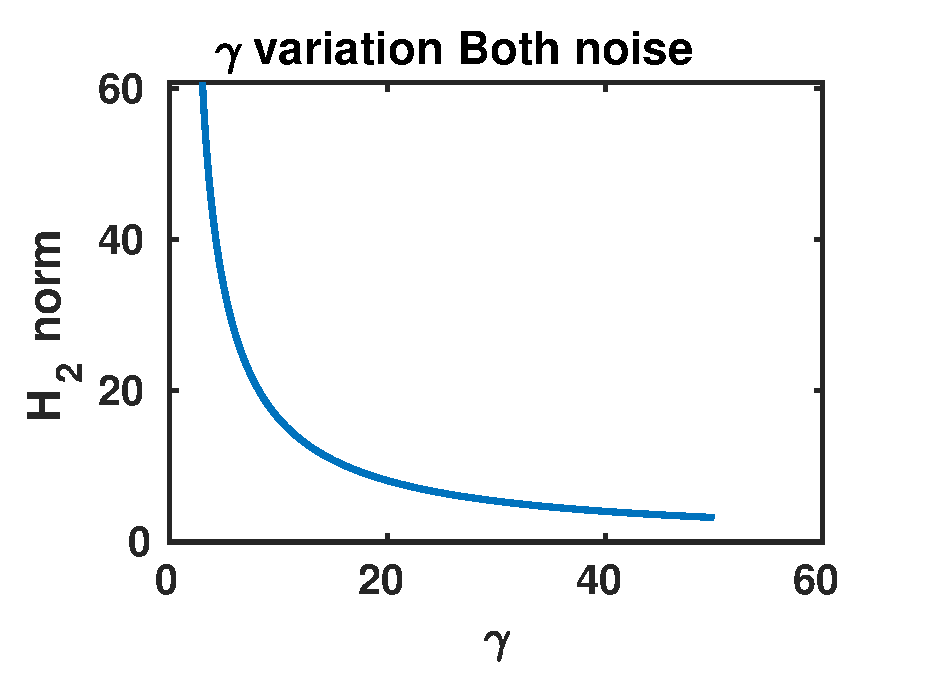
\includegraphics[scale=0.33]{Images/H2normwithgamma_Bothnoise.eps}\\
	\centering
	$\color{blue}J=2\gamma\left[2\gamma^2(I_{n-1} \otimes A_3+A_3 \otimes I_{n-1})+2I_{(n-1)^2}-(A_3^{-1} \otimes A_3+A_3 \otimes A_3^{-1})\right]^{-1}$\\
	$\color{magenta}\text{vec}(P_3)=J\text{vec}(-QQ^T)$\\
	%	\vspace{-0.4cm}
	$\color{magenta}\text{vec}(P_1)=(-1/2)(I_{n-1}\otimes A_3^{-1}+A_3^{-1} \otimes I_{n-1})\text{vec}(P_3)$\\
	$\mathcal{H}_2$ norm of the system $\color{cyan}\norm{\Sigma{\tau}}_2^2=trace(P)=trace(P_1)+trace(P_3)$\\
	\begin{block}{}
		-- The influence of $\gamma$ is encapsulated solely by $J$, and it has an inverse impact on the $\mathcal{H}_2$ performance.\\
		-- Larger values of $\gamma$ not only facilitate consensus but also help in mitigating the effects of noise.
	\end{block}
\end{frame}
%%%%%%%%%%%%%%%%%%%%%%%%%%%%%%%%%%%%%%%%%%%%%%%%%%%%
\begin{frame}{$\mathcal{H}_2$ Norm of the system with cycle length in presence of single cycle}
\begin{figure}
	\centering
	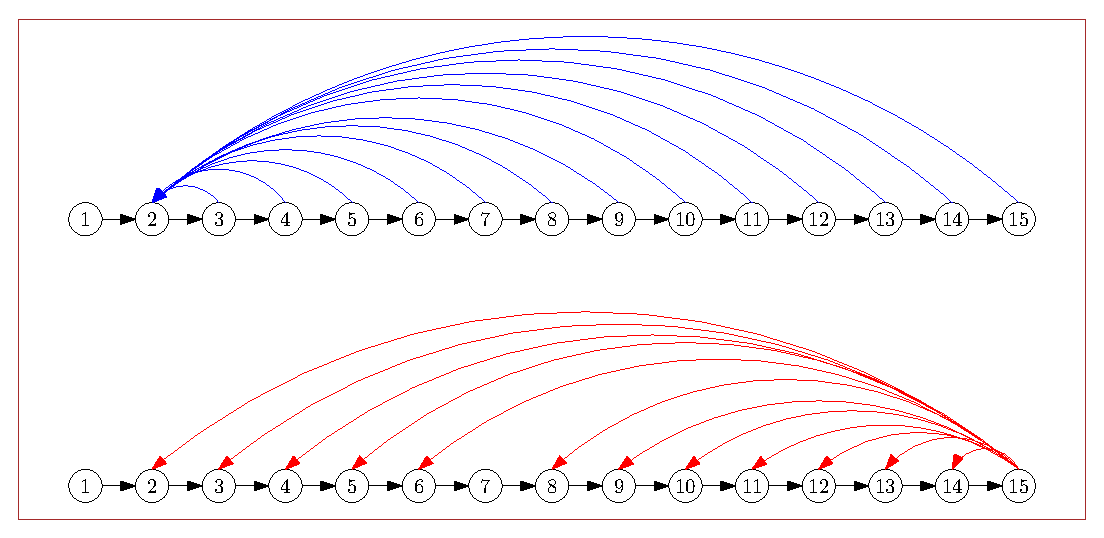
\includegraphics[scale=0.35]{Images/cycle_length.eps}
\end{figure}
\vspace{-0.5cm}
\begin{columns}
	\begin{column}{0.5\textwidth}
		%\vspace{-0.1cm}
		\begin{figure}
			%\hspace{-1cm}
			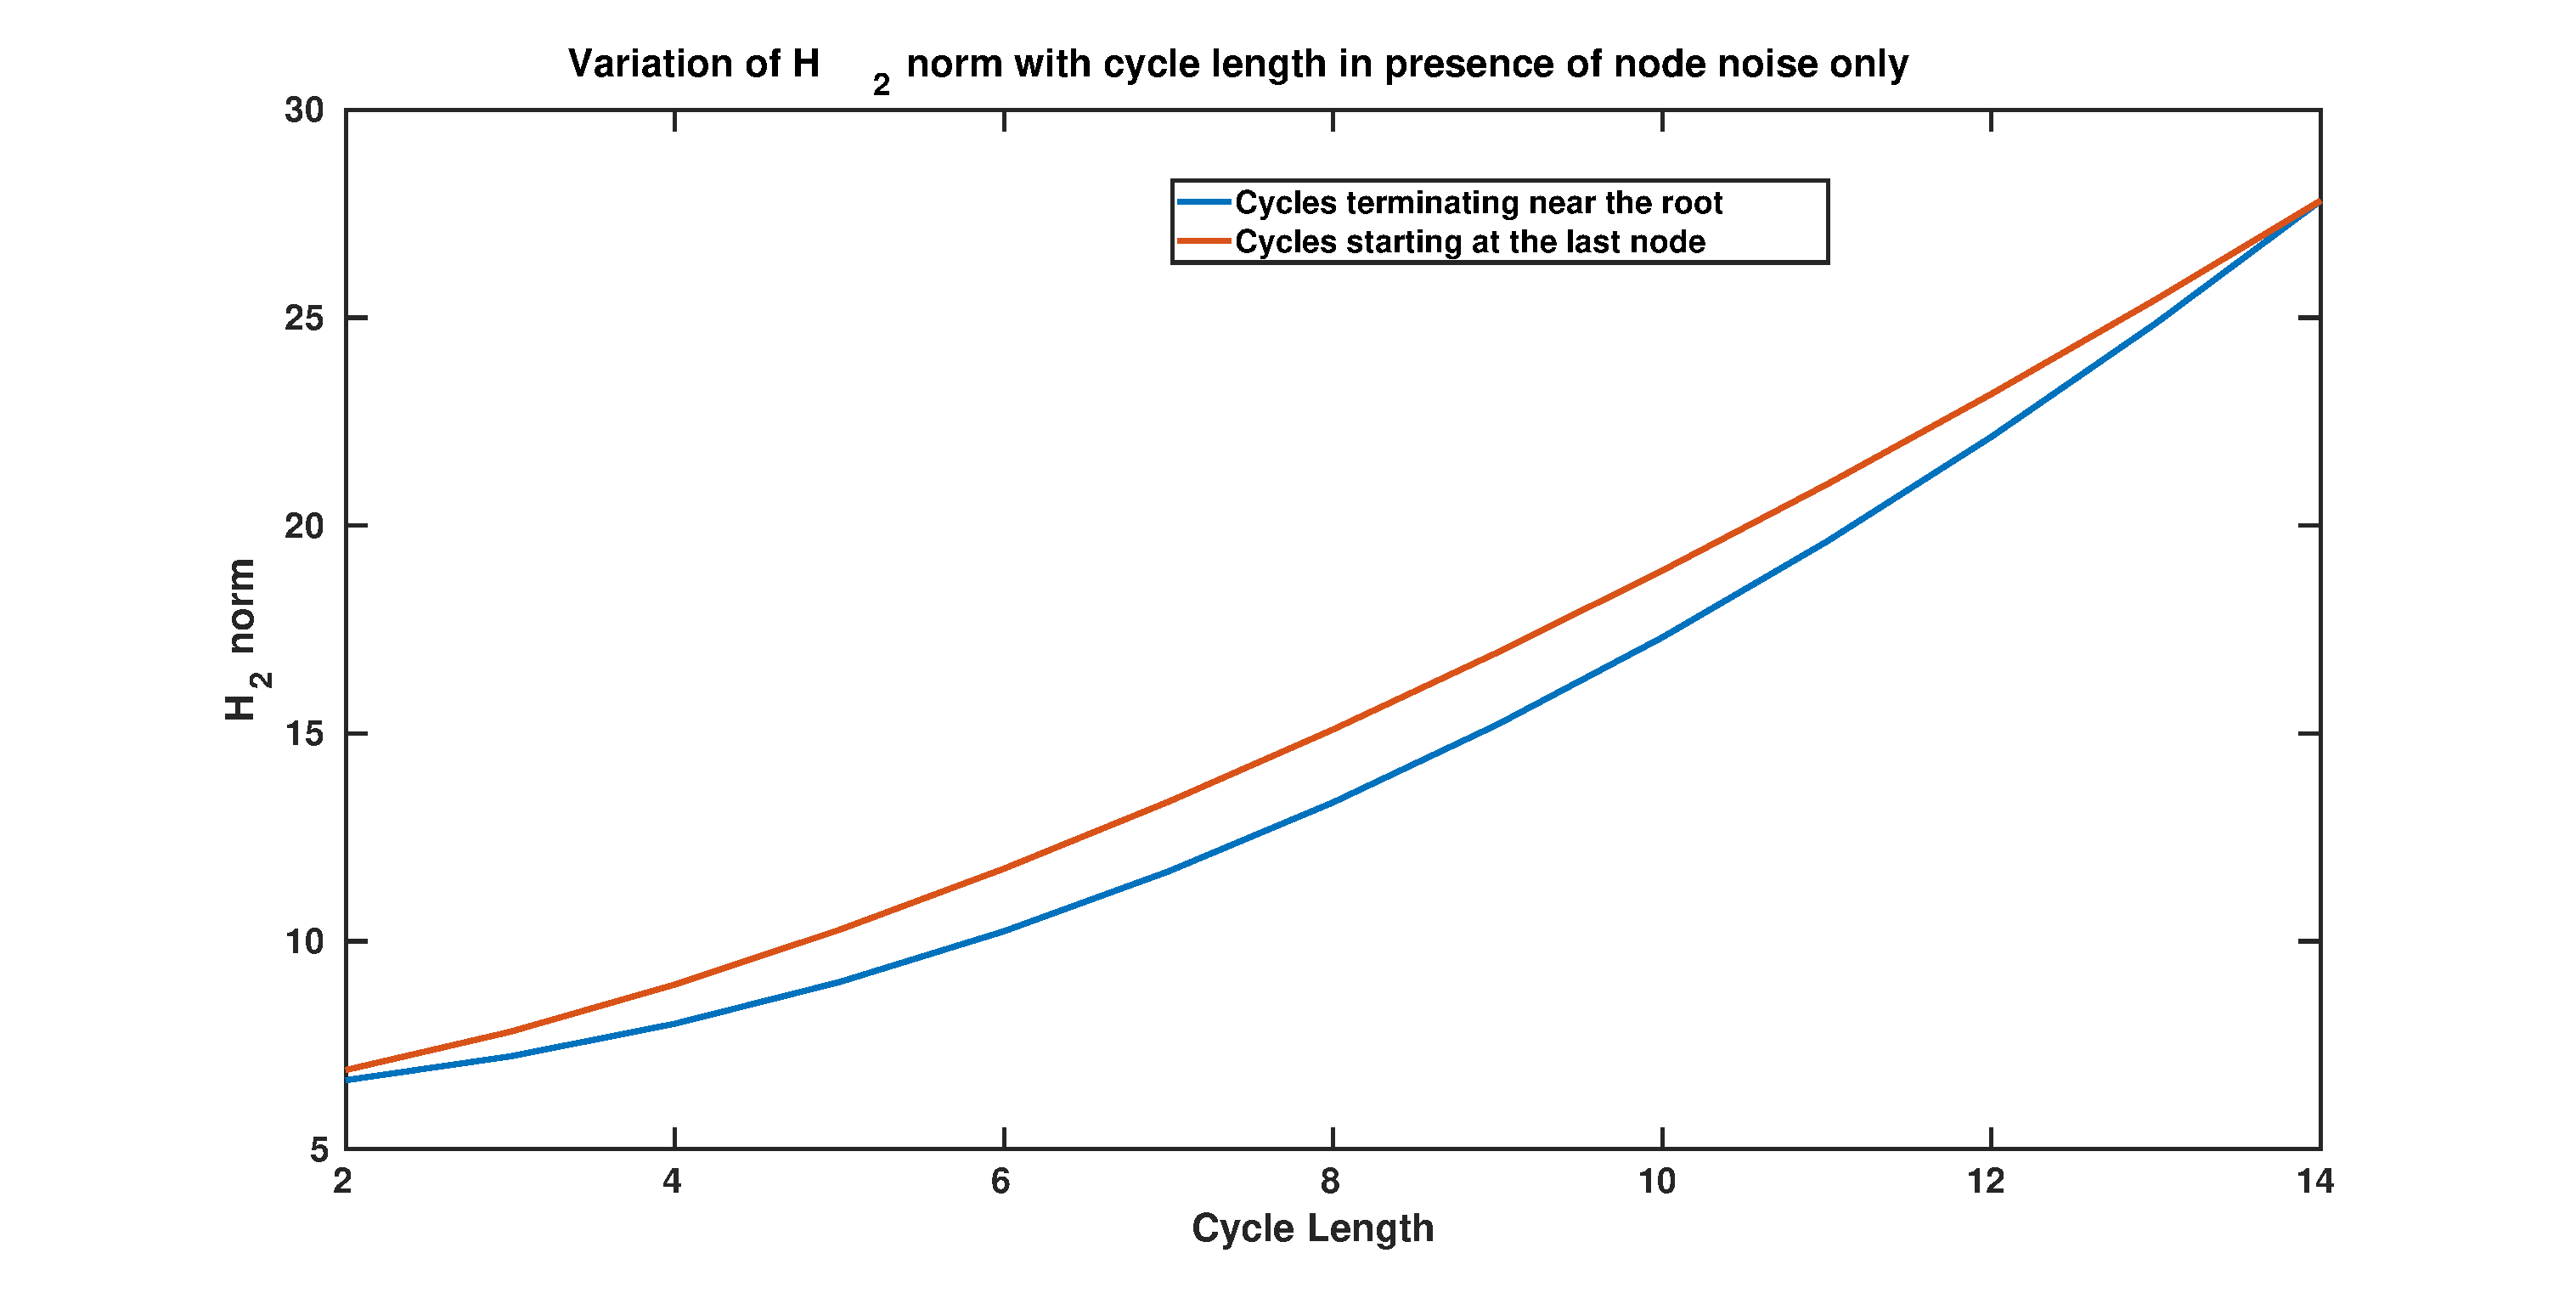
\includegraphics[scale=0.15]{Images/H2normwithcyclelength_Nodenoise.eps}
		\end{figure}
		\vspace{-0.7cm}
	\end{column}
	\begin{column}{0.5\textwidth}
		\vspace{0.5cm}
		\begin{figure}
			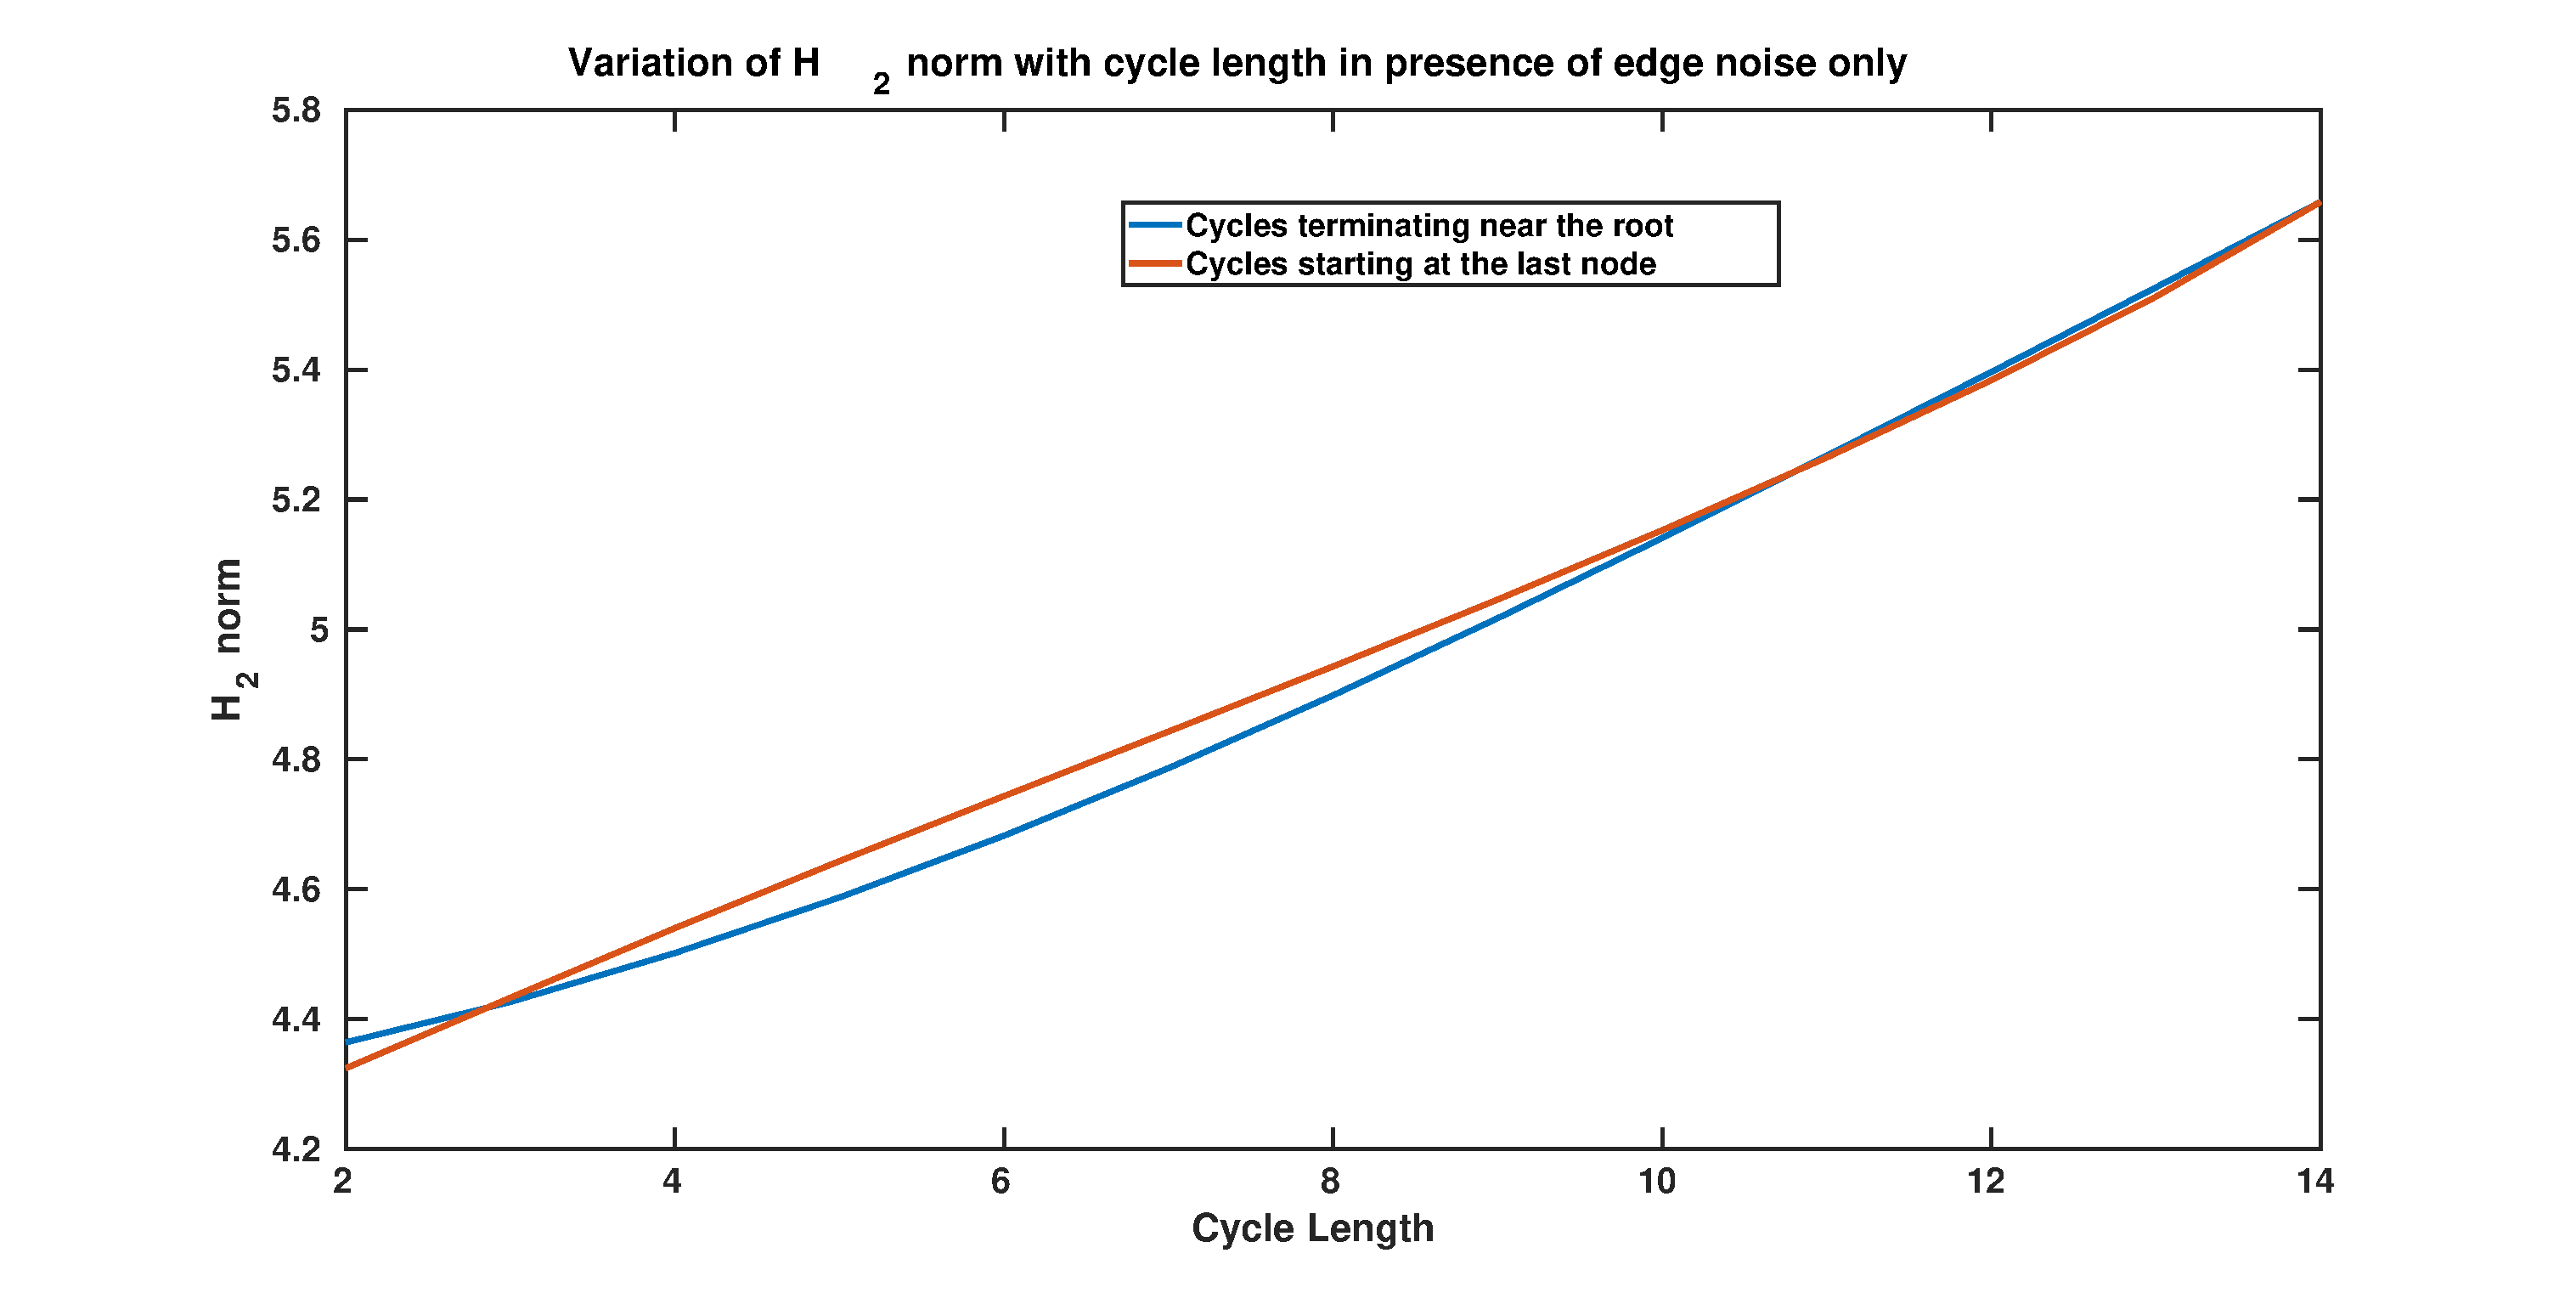
\includegraphics[scale=0.15]{Images/H2normwithcyclelength_Edgenoise.eps}
		\end{figure}
	\end{column}
\end{columns}
\vspace{-0.2cm}
\end{frame}
%%%%%%%%%%%%%%%%%%%%%%%%%%%%%%%%%%%%%%%%%%%%%%%%%%%%
\begin{frame}{$\mathcal{H}_2$ Norm of the system with cycle length in presence of single cycle}
	\begin{figure}
	\centering
	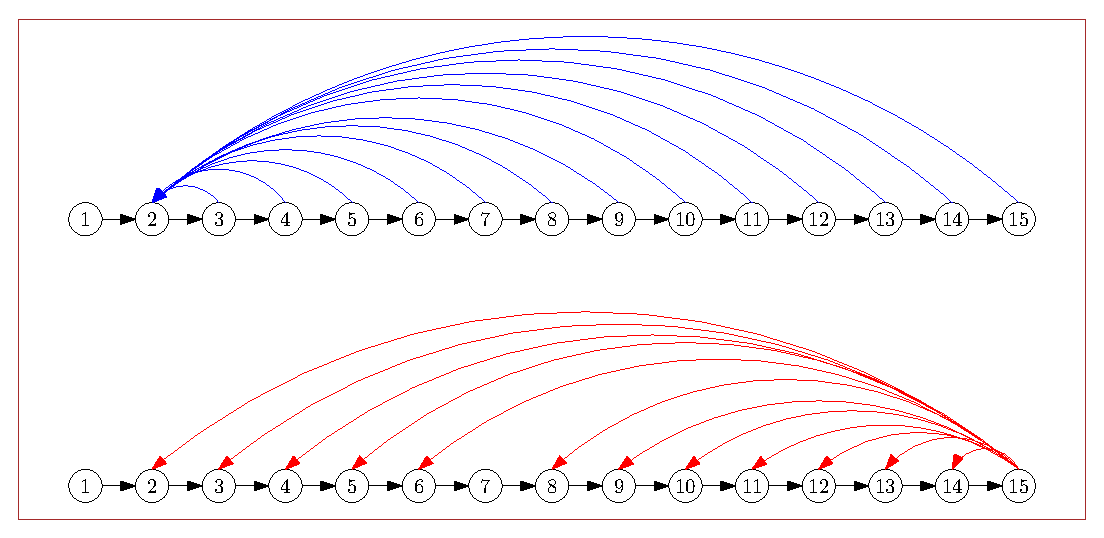
\includegraphics[scale=0.35]{Images/cycle_length.eps}
\end{figure}
\vspace{-0.5cm}
	\begin{columns}
		\begin{column}{0.5\textwidth}
			\begin{figure}
				\centering
				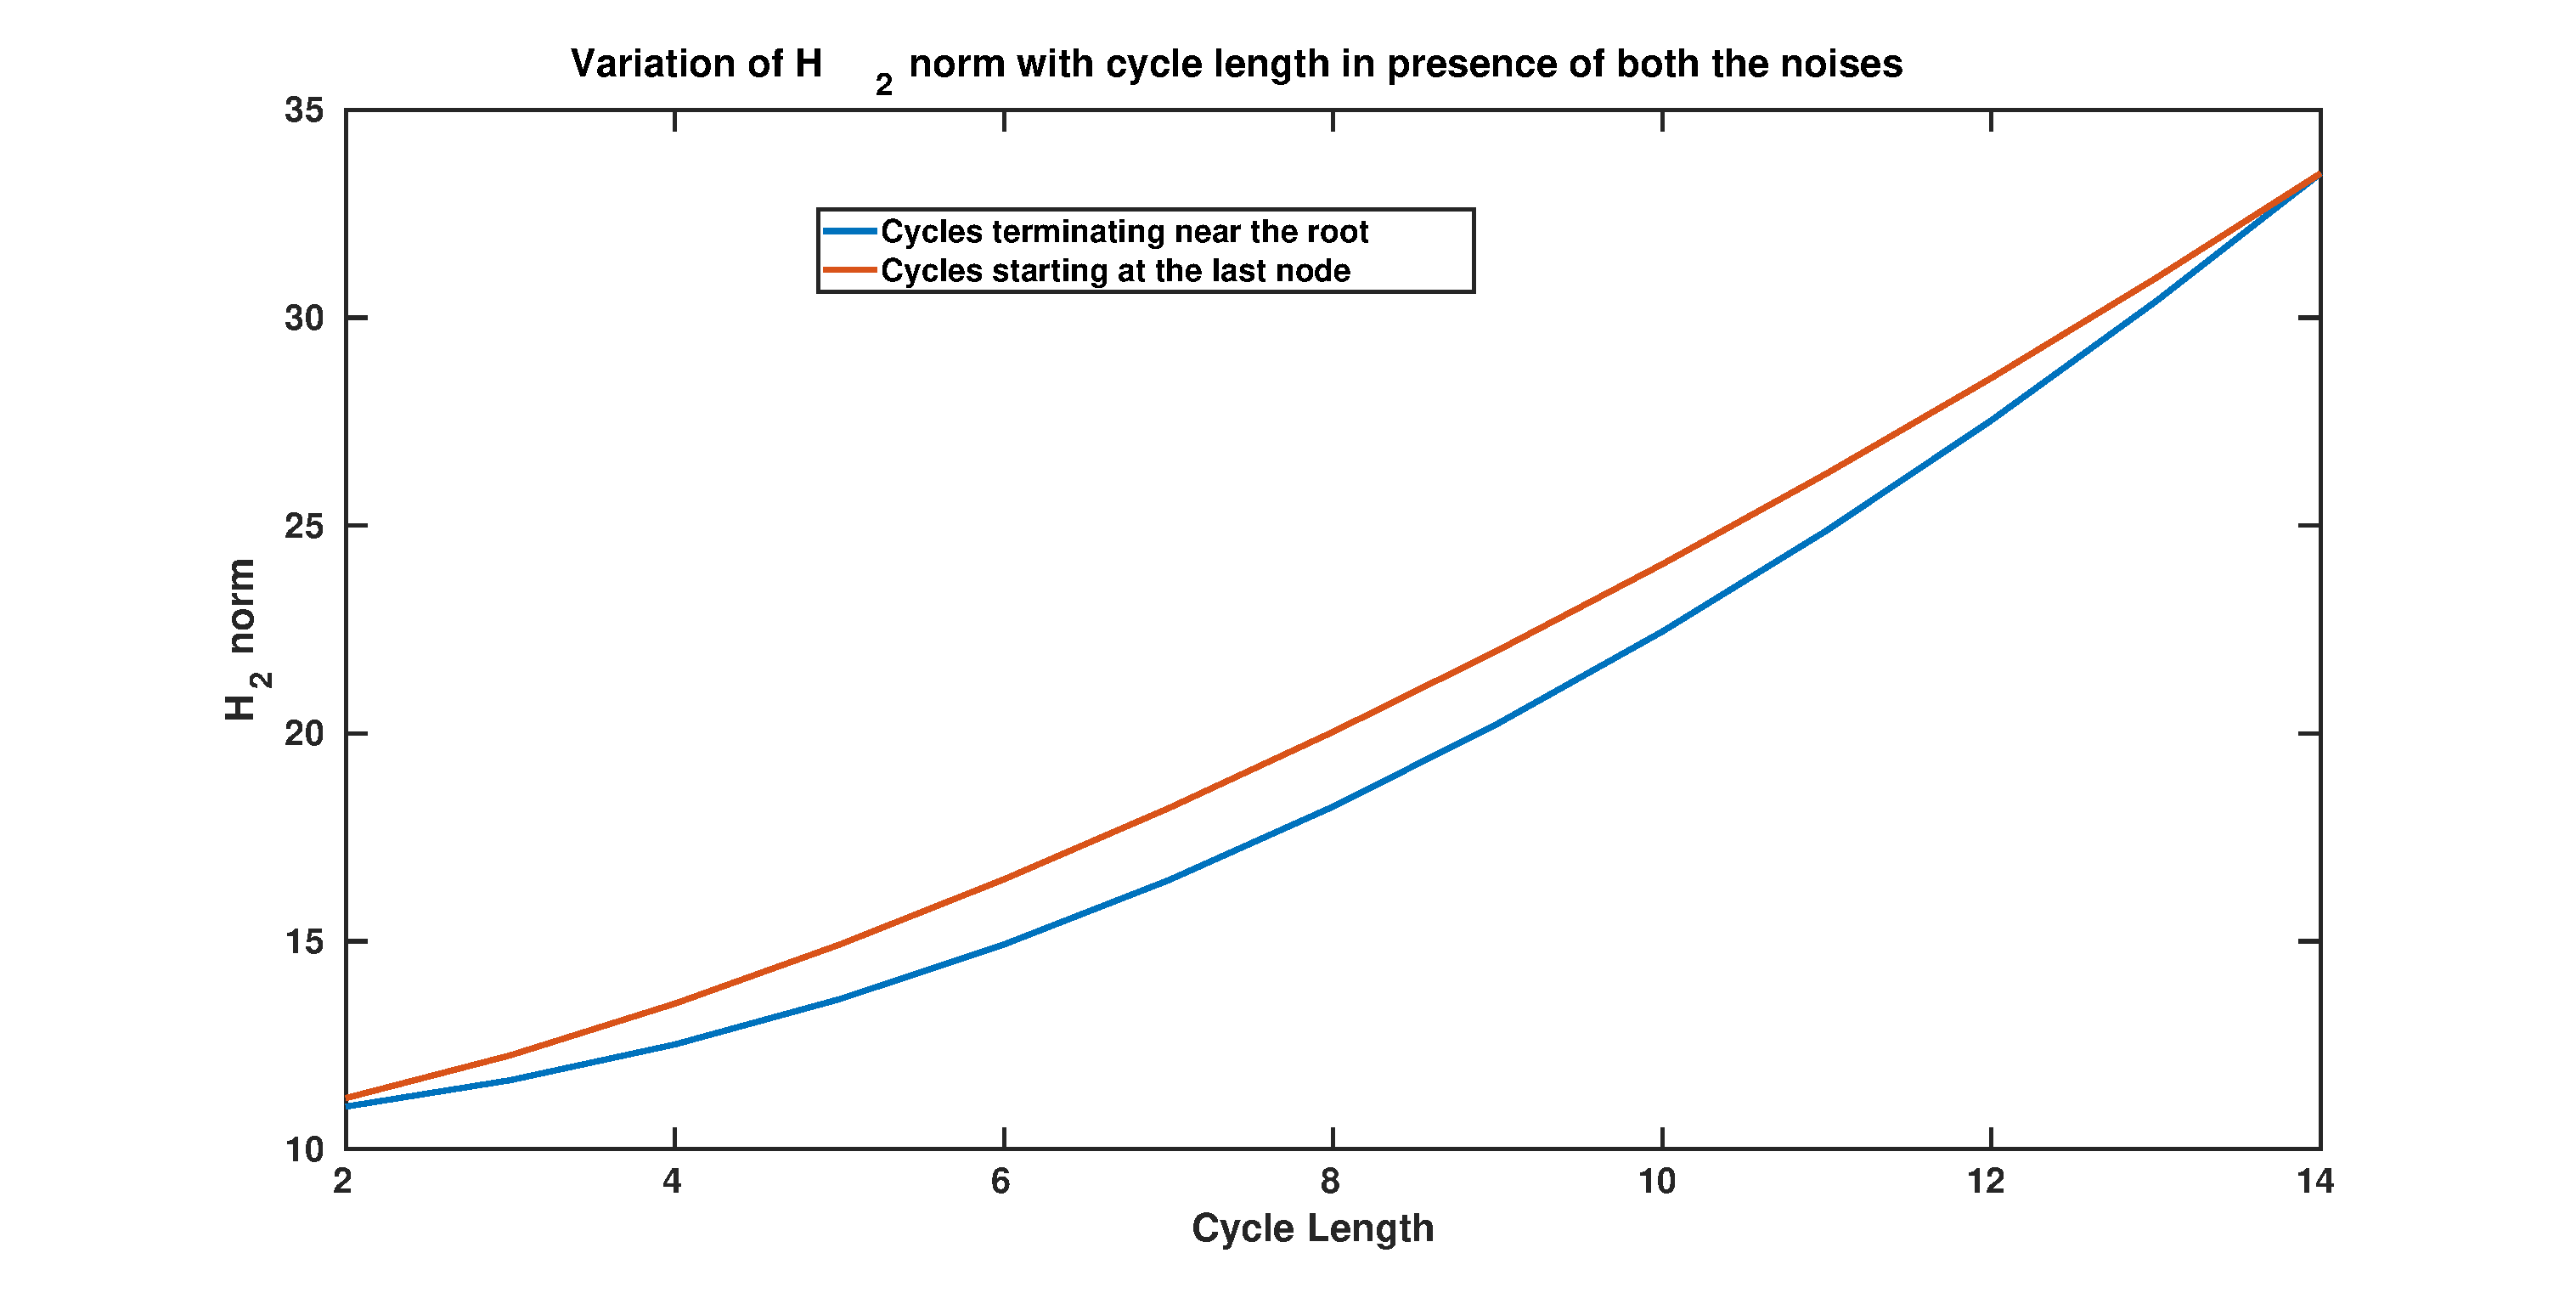
\includegraphics[scale=0.15]{Images/H2normwithcyclelength_Bothnoise.eps}
			\end{figure}
		\end{column}
		\begin{column}{0.5\textwidth}
			\begin{itemize}
				\item Cycles closer to root nodes are better.
				\item Smaller Cycles are better.
				\item Node Noise dominates the performance.
			\end{itemize} 
		\end{column}
	\end{columns}
	\vspace{-0.2cm}
\end{frame}
%%%%%%%%%%%%%%%%%%%%%%%%%%%%%%%%%%%%%%%%%%%%%%%%%%%%
\begin{frame}{$\mathcal{H}_2$ Norm of the system with varying position and cycle length}
	%\vspace{-1cm}
	\begin{columns}
		\begin{column}{0.6\textwidth}
			\vspace{-0.5cm}
			\begin{figure}
				%\hspace{-1cm}
				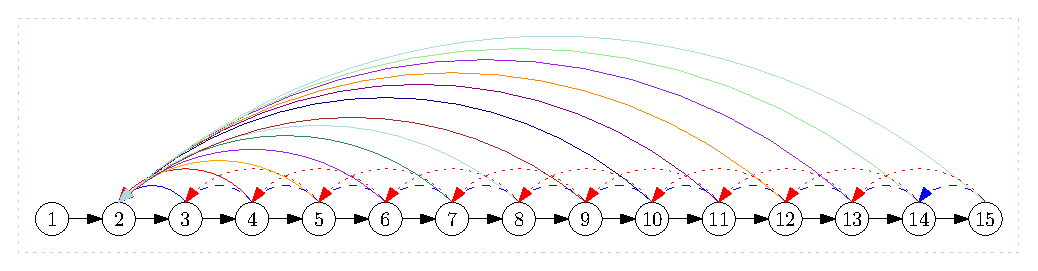
\includegraphics[scale=0.45]{Images/cycle_position_length.eps}
			\end{figure}
		\end{column}
		\begin{column}{0.5\textwidth}
			\vspace{-0.5cm}
			\begin{itemize}
				\item Performance changes with cycle position.
				\item Node Noise and Edge noise, both have positional dependence.
			\end{itemize}	
		\end{column}
	\end{columns}
	\begin{columns}
	\begin{column}{0.3\textwidth}
		\begin{figure}
			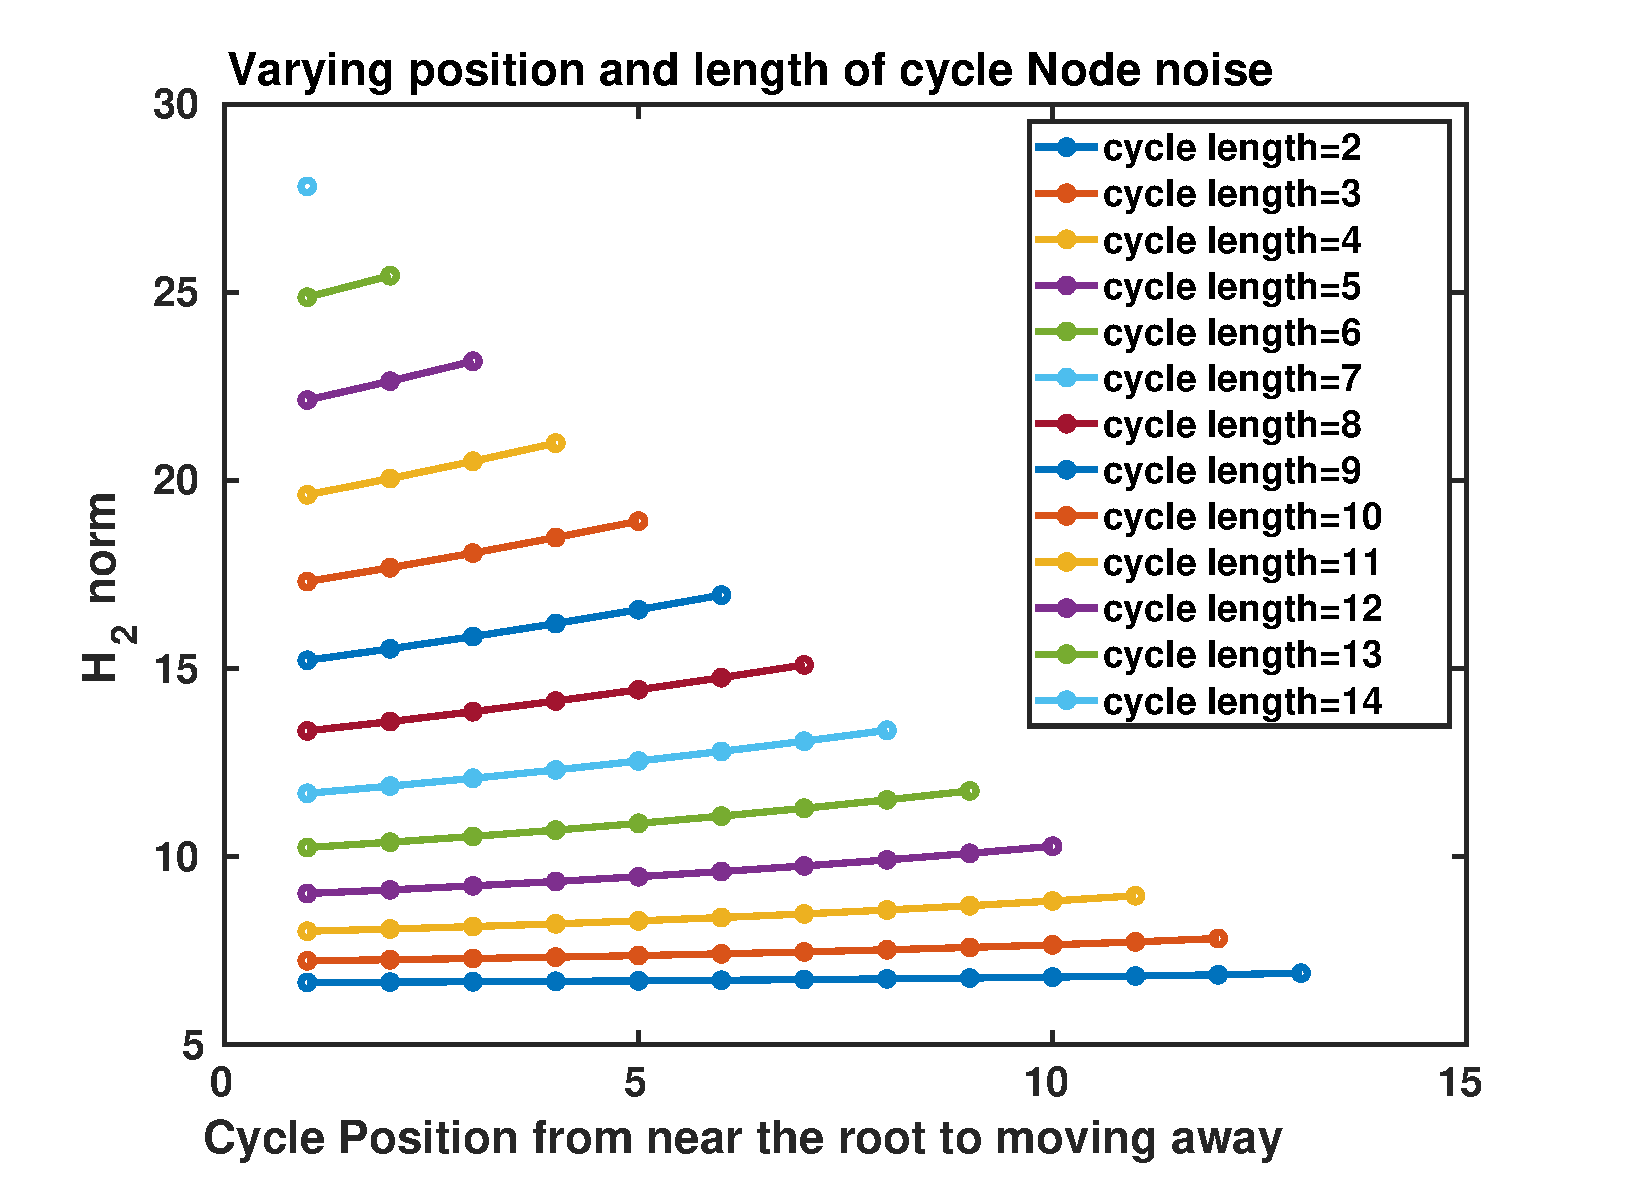
\includegraphics[scale=0.18]{Images/H2normwithvaryingcyclelengthandposition_Nodenoise2.eps}
		\end{figure}
	\end{column}
	\begin{column}{0.3\textwidth}
		\begin{figure}
			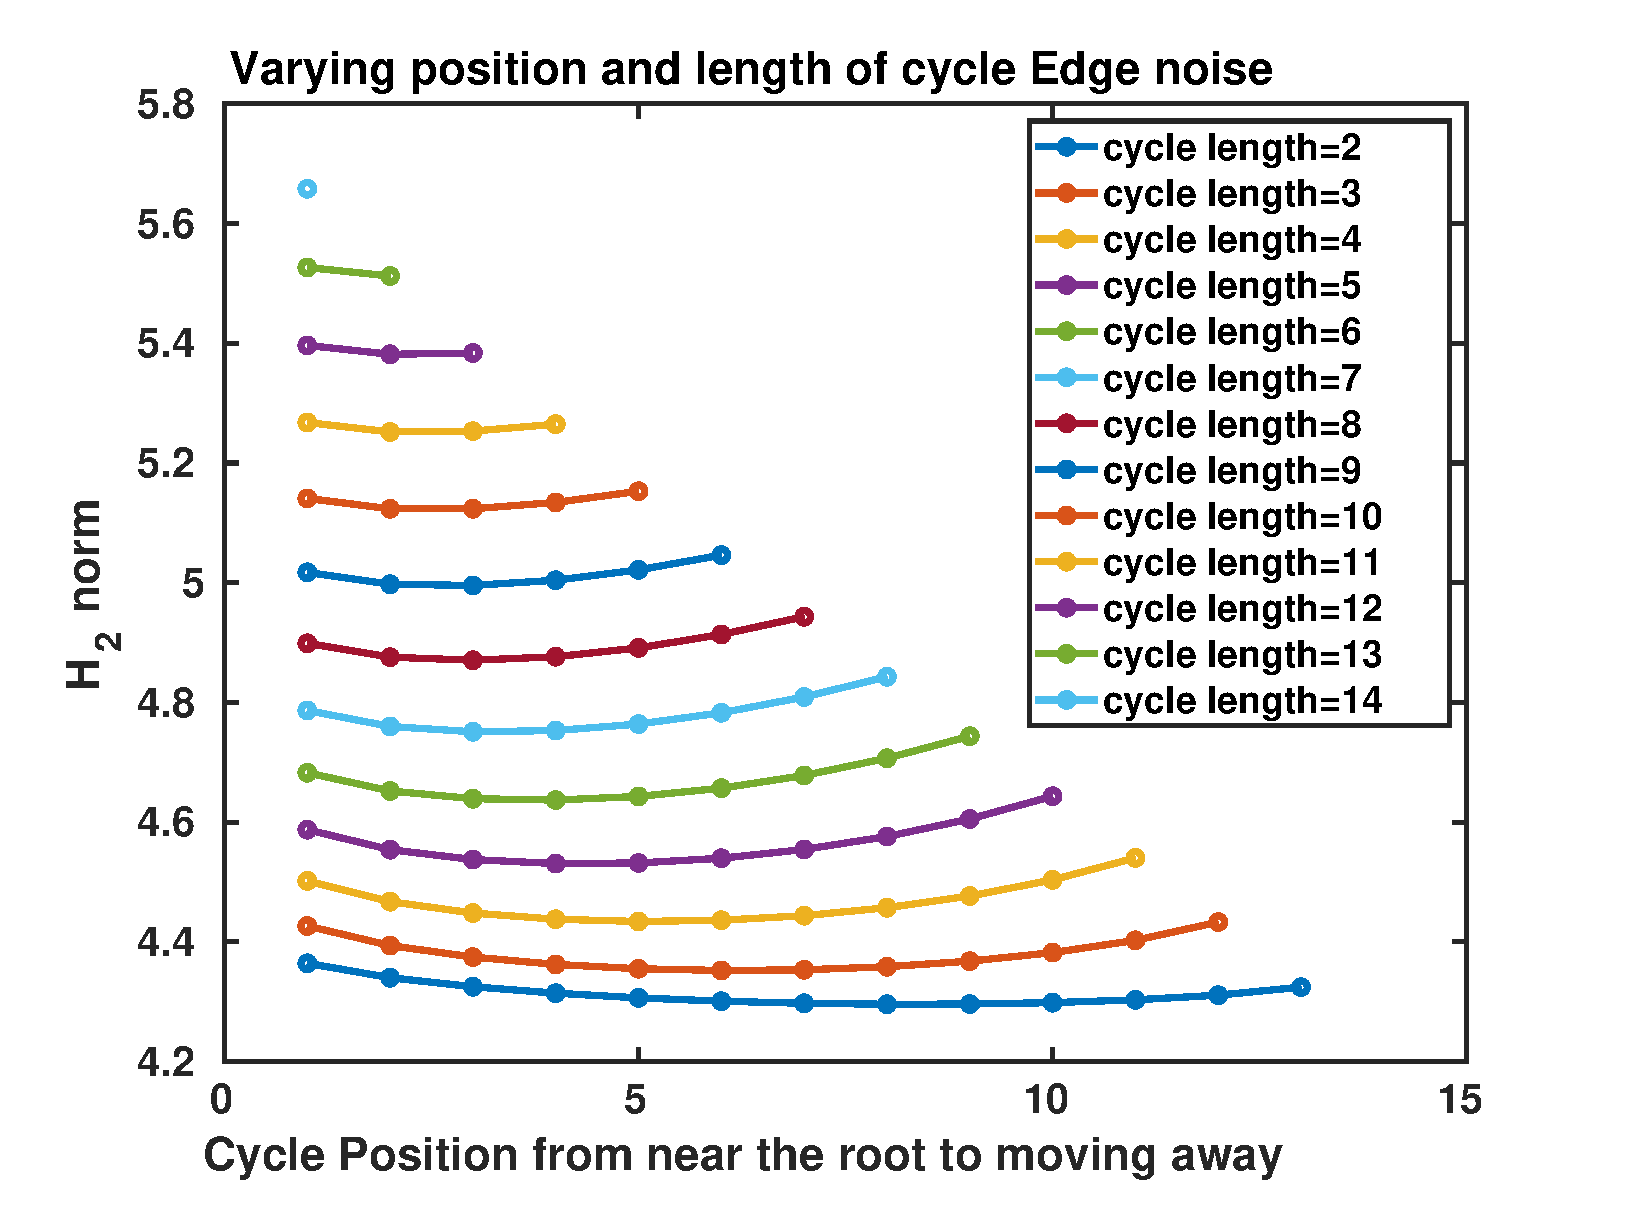
\includegraphics[scale=0.18]{Images/H2normwithvaryingcyclelengthandposition_Edgenoise2.eps}
		\end{figure}
	\end{column}
	\begin{column}{0.3\textwidth}
		\begin{figure}
			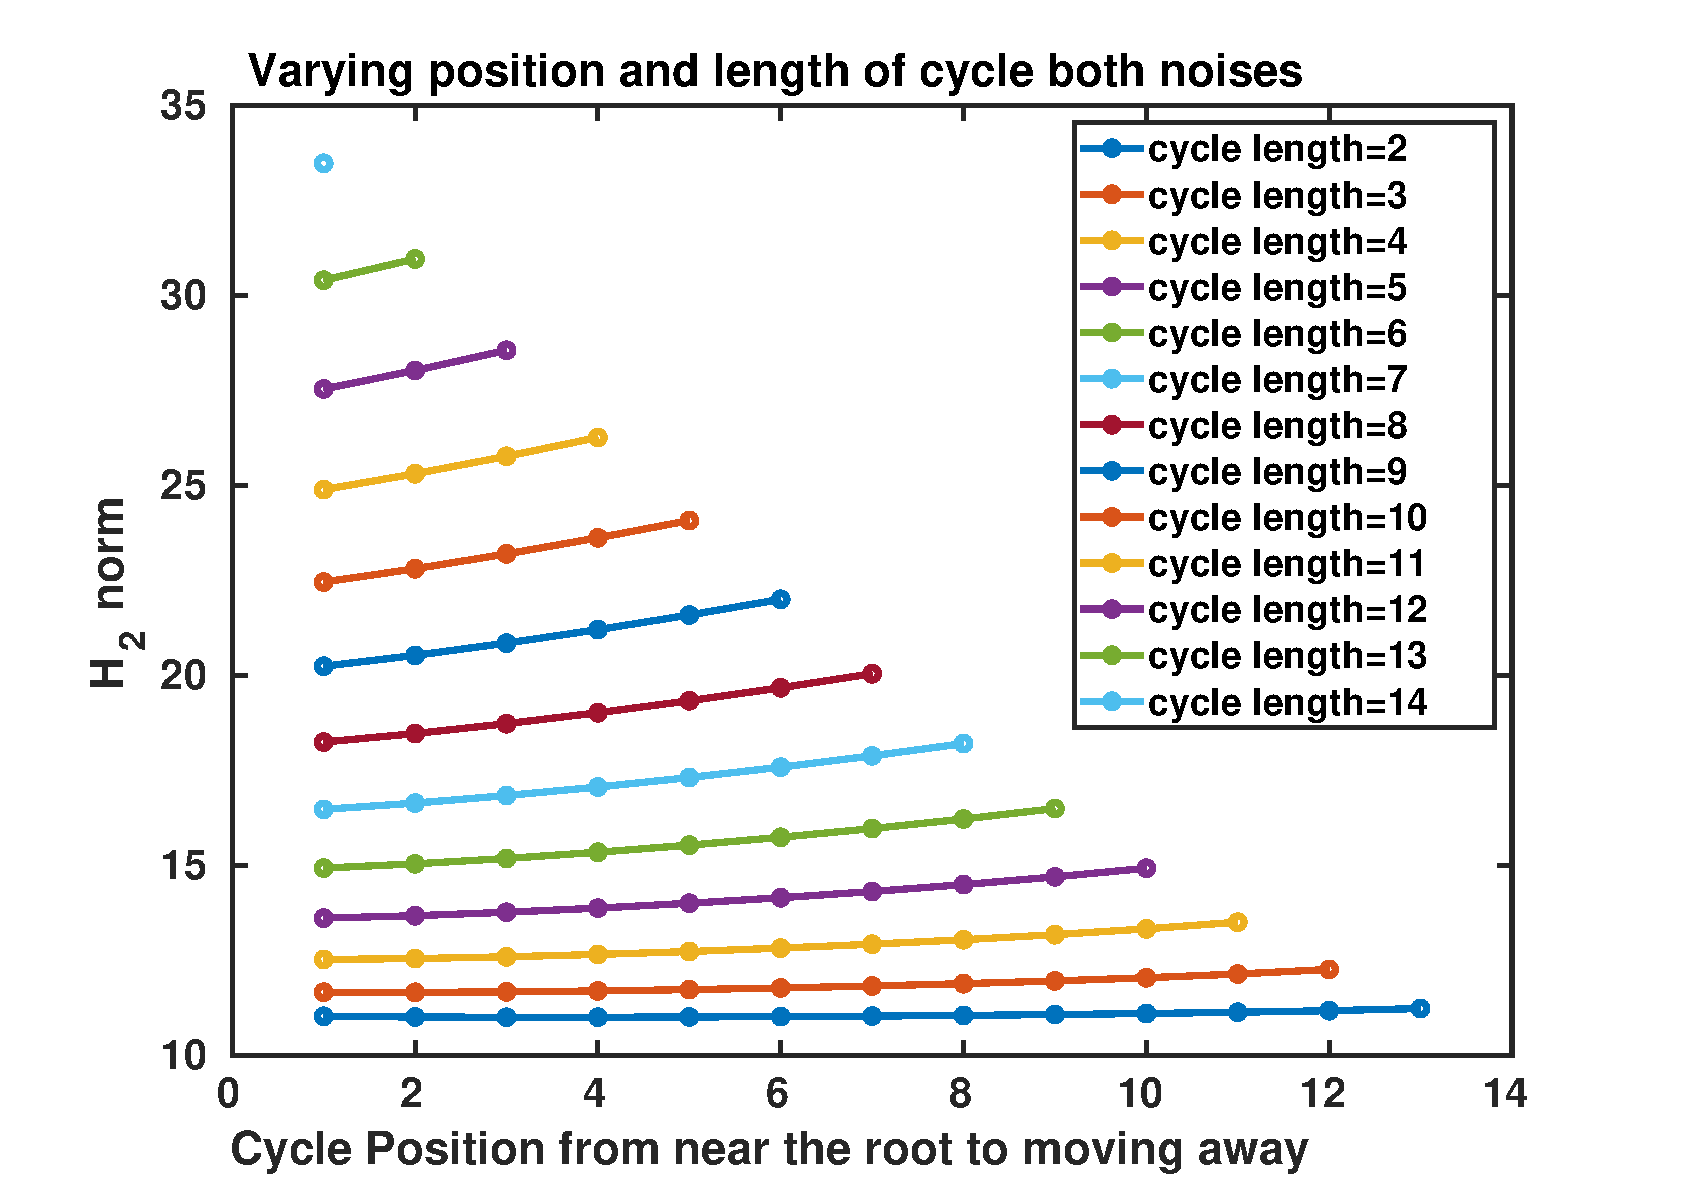
\includegraphics[scale=0.18]{Images/H2normwithvaryingcyclelengthandposition_Bothnoise2.eps}
		\end{figure}
	\end{column}
\end{columns}
\end{frame}
\end{comment}
%%%%%%%%%%%%%%%%%%%%%%%%%%%%%%%%%%%%%%%%%%%%%%%%%%%%
\begin{frame}{}
	\vspace{-0.1cm}
	\begin{block}{Conclusion}
		\begin{columns}
			\vspace{-5cm}
				% Second Column: Single Integrator Undirected Network
			\begin{column}{0.5\textwidth}
				\centering
				\textbf{Network of Single Integrators\footnotemark[1]}
				\begin{itemize}
					\item Longer cycles are better.
					\item Cycle position is not critical to performance.
					\item Choice of Spanning tree has no impact.
					\item $\gamma$ is not a parameter.
					\item Node noise and edge noise not studied separately.
				\end{itemize}
			\end{column}
			% First Column: Double Integrator Directed Network
			\begin{column}{0.5\textwidth}
				\centering
				\textbf{Network of Double Integrators}
				\begin{itemize}
					\item Longer cycles are better.
					\item Cycles at the center of tree are better.
					\item Choice of Spanning tree affect the performance.
					\item Larger values of $\gamma$ are better
					\item Node noise results in variation with cycle position.
				\end{itemize}
			\end{column}
		\end{columns}
	\end{block}
	\footnotetext[1]{\textcolor{blue}{Zelazo, Daniel, Simone Schuler, and Frank Allgöwer.}, {\em "Performance and design of cycles in consensus networks." Systems \& Control Letters 62.1 (2013): 85-96.}}
\end{frame}
\begin{comment}
	\pause
	\begin{block}{Future Work}
		\begin{itemize}
			\item Find analytical solution for directed network.
			\item Study the effects of multiple cycles in the network.
		\end{itemize}
	\end{block}
	
	\vspace{-0.2cm}
		% Second Column: Single Integrator Undirected Network
	\begin{column}{0.35\textwidth}
		\centering
		\textbf{Second Order Directed}
		\begin{itemize}
			\item Shorter cycles are better.
			\item Cycles closer to the root node are better.
			\item Choice of Spanning tree affect the performance.
			\item Larger values of $\gamma$ are better.
			\item Both noises result in positional dependence with Node noise dominating the performance.
		\end{itemize}
	\end{column}
\end{comment}
%%%%%%%%%%%%%%%%%%%%%%%%%%%%%%%%%%%%%%%%%%%%%%%%%%%%